%----------------------------------------------------------------------------------------
%	PACKAGES AND OTHER DOCUMENT CONFIGURATIONS
%----------------------------------------------------------------------------------------

\documentclass[
11pt, % Sjors Was Here The default document font size, options: 10pt, 11pt, 12pt
%oneside, % Two side (alternating margins) for binding by default, uncomment to switch to one side
english, % ngerman for German
singlespacing, % Single line spacing, alternatives: onehalfspacing or doublespacing
%draft, % Uncomment to enable draft mode (no pictures, no links, overfull hboxes indicated)
%nolistspacing, % If the document is onehalfspacing or doublespacing, uncomment this to set spacing in lists to single
% liststotoc, % Uncomment to add the list of figures/tables/etc to the table of contents
%toctotoc, % Uncomment to add the main table of contents to the table of contents
%parskip, % Uncomment to add space between paragraphs
%nohyperref, % Uncomment to not load the hyperref package
headsepline, % Uncomment to get a line under the header
%chapterinoneline, % Uncomment to place the chapter title next to the number on one line
%consistentlayout, % Uncomment to change the layout of the declaration, abstract and acknowledgements pages to match the default layout
]{MastersDoctoralThesis} % The class file specifying the document structure

\title{Development of an Omni-directional distance sensing module for the Deci Zebro}

\usepackage[utf8]{inputenc} % Required for inputting international characters
\usepackage[T1]{fontenc} % Output font encoding for international characters
\usepackage{mathtools}
\usepackage{times} % Use times format
\usepackage{abstract}
\usepackage[hidelinks]{hyperref}
\usepackage{float}
\usepackage{enumitem}% http://ctan.org/pkg/enumitem
\usepackage[official]{eurosym}
\usepackage[style=ieee]{biblatex}
	\addbibresource{lit.bib}
\usepackage[autostyle=true]{csquotes} % Required to generate language-dependent quotes in the bibliography
\usepackage{enumitem} %For the table of req.
\setlist[enumerate]{label*=\arabic*.}
\usepackage{caption}
\usepackage{subcaption}
\usepackage{pdfpages}
\usepackage{eurosym}



\newenvironment{reqs}[1]{
  \def
	\reqletter{#1}
  \begin{enumerate}
      [label={\bfseries [\reqletter-\arabic{enumi}]},
       beginpenalty=0, midpenalty=50, endpenalty=0]
			 }
{\end{enumerate}}

\newenvironment{subreqs}{
  \begin{enumerate}
      [label={\bfseries [\reqletter-\arabic{enumi}.\arabic{enumii}]},
       beginpenalty=100, midpenalty=100, endpenalty=0]
}
{\end{enumerate}}

%----------------------------------------------------------------------------------------
%	MARGIN SETTINGS
%----------------------------------------------------------------------------------------

\geometry{
	paper=a4paper, % Change to letterpaper for US letter
	inner=3.3cm, % Inner margin
	outer=3cm, % Outer margin
	bindingoffset=.5cm, % Binding offset
	top=1.5cm, % Top margin
	bottom=1.5cm, % Bottom margin
	%showframe, % Uncomment to show how the type block is set on the page
}


\begin{document}

\frontmatter % Use roman page numbering style (i, ii, iii, iv...) for the pre-content pages

\pagestyle{plain} % Default to the plain heading style until the thesis style is called for the body content

%----------------------------------------------------------------------------------------
%	TITLE PAGE
%----------------------------------------------------------------------------------------


 \begin{titlepage}

	\vspace{1cm}
	{\scshape\Large Electrical Engineering Bsc. Thesis\par}
	\vspace{1cm}
	{\huge\bfseries Development of an Omni-directional\par distance sensing system for the\par Deci Zebro\par}
	\vspace{1.5cm}
	K. Kouwenhoven (4222849) \par S. G. Verkamman (4294815)\par
	\vspace{1.5cm}
  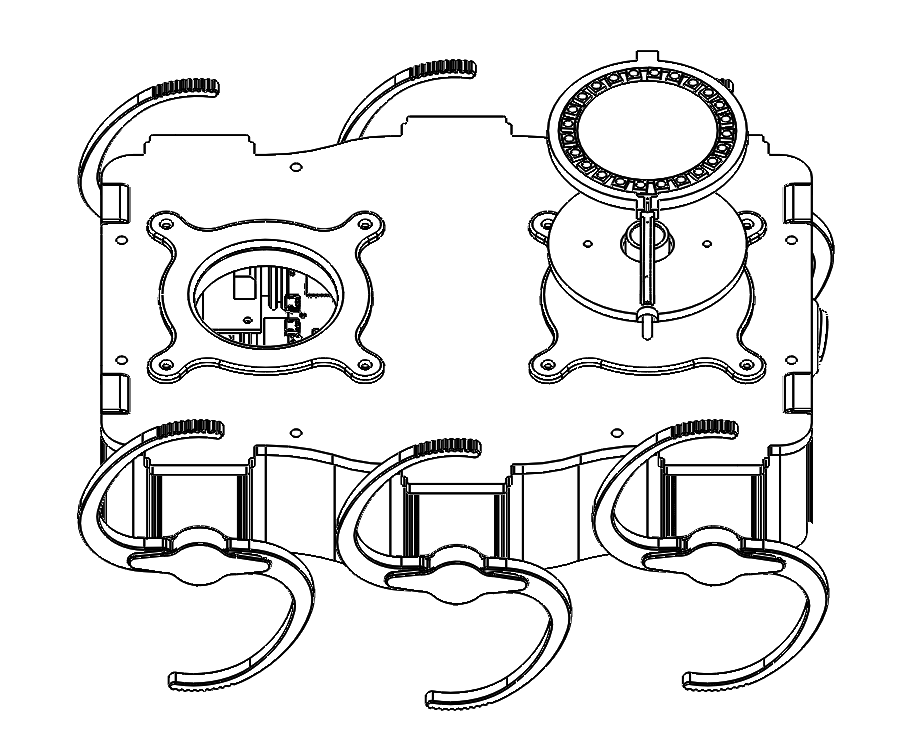
\includegraphics[width=\textwidth]{Figures/zebro_black_white.PNG}\par
	\vfill
	% Bottom of the page
	{\Large Supervisors:\par}
	Chris Verhoeven (EWI, TuDelft)\par
	Edwin Hakkennes (EWI, TuDelft)\par
	Ronald Bos (EWI, TuDelft)\par
	Daniël Booms (The Zebro project, TuDelft)\par
	\vspace{1cm}
	{\scshape\large Technische Universiteit Delft\par}
	{\large June 2017}
 \end{titlepage}

%----------------------------------------------------------------------------------------
%	ABSTRACT PAGE
%----------------------------------------------------------------------------------------

\begin{abstract}
\addchaptertocentry{\abstractname} % Add the abstract to the table of contents
In this thesis, we describe the design process of a distance sensing system for the Deci Zebro swarm robots.
We use a technique that transmits a radio frequency message and a ultrasonic pulse concurrently.
Due to the difference in propagation speed of both signals, the distance could be measured using time difference of arrival (TDOA).
A cone shaped antenna is designed to create a \SI{360}{\degree} ultrasonic pulse coverage.
At the end of this thesis we present a prototype with a range of \SI{7}{\meter}.
We find a linear relation between the TDOA and the actual distance between the modules.
We thus conclude that our prototype is suitable for range measurements on roving swarm robots.
\end{abstract}

%----------------------------------------------------------------------------------------
%	LIST OF CONTENTS/FIGURES/TABLES PAGES
%----------------------------------------------------------------------------------------

\tableofcontents % Prints the main table of contents

%\listoffigures % Prints the list of figures

%\listoftables % Prints the list of tables

%----------------------------------------------------------------------------------------
%	CHAPTERS
%----------------------------------------------------------------------------------------

\mainmatter% Begin numeric (1,2,3...) page numbering

\pagestyle{thesis} % Return the page headers back to the "thesis" style

\chapter{Introduction}

The ZEBRO project is a swarm robotics research group at the TU Delft.
Its mission is:
\\\\
\emph{To develop self-deploying, inexpensive, extremely miniaturised and autonomous roving robots which cooperate in swarms capable of functioning in a wide spectrum of topologies and environments that can quickly provide information with the help of distributed sensor systems and supports payloads suitable for a wide range of missions.}
\\\\
Zebro started in September 2013, and has now been absorbed by the TU Delft Robotics Institute as part of their research endeavours into swarm robotics.

The idea of swarm robotics is inspired by nature, in particular by small insects or birds who exhibit so-called swarm behaviour.
As a group, the swarm can accomplish complex tasks, despite the fact they are not considered `smart' individually.
By all following the same simple set of rules, the swarm as a whole can exhibit emergent behaviour, behaviour that is not explicitly programmed into any one of its members.
For example, flocking is not the behaviour of a single bird but the emergent behaviour of the entire flock.

This idea that a group of simple individuals can deal with more complex tasks is the cornerstone of swarm robotics.
Furthermore, an entire swarm is very resilient, as every individual member is expendable.
This means that swarm robotics has some unique applications, such as in a disaster area that is inaccessible to humans or large robots, due to a hazardous or arduous environment.

Currently, the ZEBRO project is working to redesign the robots to (further) improve producibility, reparability, stability, and lower unit cost.
Being able to produce useful ZEBRO units on a large scale will provide fertile ground for swarm robotics research efforts.
There are several different versions of the ZEBRO, each with a different form factor and design goal.
Our research focuses on the Deci ZEBRO, which is the size of an A4 sheet of paper and is designed to be extremely modular.

Our group's goal is the design of a communication and localisation module for the Deci Zebro.
The module has two purposes.
The first is to provide a Zebro robot with the positions of robots in its vicinity.
The second is to facilitate wireless communication within the Zebro swarm.

Localisation is done by using range measurements.
This has lead to the following subdivision of our module:
\begin{itemize}
  \item
    The \textbf{distance sensing} system measures the distance between Zebro robots.
  \item
    The \textbf{communication} system sets up a decentralised mesh network for communication.
  \item
    The \textbf{processing} system takes the measurements provided by the other submodules and uses them to construct a local (i.e.\ in the Zebro's neighbourhood) model of the swarm.
\end{itemize}

This Thesis focusses on the design of the distance sensing submodule for the Deci Zebro.

\section{Problem definition}

We need to design a system that can measure the distance between robots operating in a swarm.
The system should provide the Zebro `brain` a distance and an angle with a certain accuracy.
This distance has to be matched to a Zebro serial number such that the `brain` knows to which Zebro the range and angle relates.
For this thesis we will elaborate the range determining subsystem that should provide a distance with a certain accuracy to the central processor of the localisation and communication module.
The central processes will perform the processing action and presents the data, in the correct format, to the Zebro `brain`.

\section{State of the art}

For the distance sensing functionality of the Zebro we are looking into a technique that uses off the shelf devices, such as Bluetooth modules, and is capable of giving accurate distance measurements on a moving robot.
As a start we found two documents \cite{Ekberg2009,Kuriakose2014} explaining the general concept of localisation and the usable techniques.
Using these documents we set out to research on the topics of Received signal strength indicator (RSSI), Time of flight and time difference of arival (TDOA) as distance sensing techniques and finding the possible implementations of them.
The results are given in the following subsections:

\subsection*{Bluetooth}

Bluetooth devices have two usable standard parameters: Received signal strength indicator (RSSI) and link quality. Both could be used to determine the distance between devices since, in theory, both parameters linearly depend on the distance between devices. Literature shows that using know formulas, the distance between devices can be estimated from the RSSI. Literature \cite{Forno2005} shows two problems with using RSSI as a distance sensing technique: the RSSI is not stable since the Bluetooth protocol takes measures to ensure the highest quality link and the RSSI is dependent on device orientation. Papers \cite{Scheerens2012,Dahlgren2014} gives values for the orientation dependency: in worst case the result for a measurement done at 1 meter distance gives a RSSI values which corresponds to 10 meter. Using RSSI for distance sensing might be possible in static environments with fixed device orientation but is not adequate in a system with moving devices.

Another possibility for using Bluetooth in distance sensing is measuring the time-of-flight of transmitted messages. We can either measure the time difference between sending a message and when it arrives at the other device or we can measure the round trip time when a message is transmitted back and forth between two devices. For the first method both devices would need high accuracy synchronised clocks \cite{Ekberg2009} and the second methods is highly dependent on both the message processing time and the accuracy of the internal clock. Furthermore the technique is difficult to implement in a system where messages are hopped between robots making it hard to determine which path the message has travelled.

\subsection*{Radio Frequency}

It is possible to determine the angle of arrival (AOA) using rotating directional antenna's, antenna arrays or beam forming antenna \cite{Min2016}. This (AOA) could be used to map devices and estimate the distance between these mapped devices based on received signal power. The problem is that these systems are big, expensive and complex making them unfavourable for use on a Zebro and within the time frame of the BAP.

\subsection*{Acoustic}

Acoustic signals \cite{Peng2007} can be used to determine the time-of-arrival (TOA). Two-way sensing is used to determine the distance without the need for synchronised clocks. The result is a low cost, high accuracy device which operates in the audible sound spectrum. The range for indoor applications is roughly 5 meters due to reflection/multipath.

\subsection*{Infra red}

The paper about the Multirobot Positioning Systems \cite{Pugh2009} describes a system of miniature robots which use IR to determine the distance between robots. The range of this system is around 3 meters.

\subsection*{Ultrasonic}
MIT has designed an indoor location-support system called Cricket \cite{Priyantha2000,Priyantha2005,Balakrishnan2003,Smith2005}, that uses ultrasound in combination with the RF communication channel to determine distance between two devices.
The system measures the time difference of arrival (TDOA) of a RF transmitted ID tag and an ultrasonic pulse.
This time difference is related to the distance and gives results with an accuracy of 1 cm with proper filtering techniques. This system uses beacons with a fixed position to determine the relative distance of moving devices.
The range of the system is roughly 10 meters.

The Cricket team has used two methods to detect if the system receives an ultrasonic pulse. The first is a phase locked loop (PLL) as discussed in \cite{Hsieh1996}.
The PLL tracks the incoming signal and produces as synchronised output signal.
This output signal has the same phase, and thus frequency, as the incoming signal.
Since the frequency of the ultrasound pulse is known a tone detector can be used to detect the frequency of the synchronised output signal.
If the frequency of the synchronised signal is the same as the frequency of the transmitted ultrasonic pulse the system is receiving an ultrasound pulse.

The second method is to use a peak detection circuit to detect the amplitude of the incoming signal as describe in \cite{Bhagat2015}.
The peak detection circuit charges and discharges a capacitor creating a voltage level corresponding to a certain amplitude.
This voltage level can than be detect by, for example, an comparator.

\subsection*{Conclusion}

At this point in the literature study we see the most potential in a system using ultrasound and the communication channel. Both the accuracy and the range are high. Other researched systems fall short on one of these fronts: Bluetooth systems have a high range but the accuracy for moving devices is poor, acoustic and IR systems have a high accuracy but the range is insufficient for the Zebro swarm.

The biggest challenge of a ultrasonic system is the directional nature of ultrasonic transmitters and receivers. In the Zebro swarm we need a distance sensing system with a 360 degree field. Using the ultrasonic reflector antenna \cite{Claycomb1992} a omnidirectional ultrasonic transducer is created, which allows us to create a mobile version of the cricket system \cite{Priyantha2000,Priyantha2005,Balakrishnan2003,Smith2005} usable for the Zebro swarm.


\section{Thesis synopsis}

The main body of the thesis, which focusses on the design phase, is divided in three main parts:

\begin{itemize}
  \item
  \textbf{The conceptual design} in this part the used concept will be described.
  This concept will then be further refined into subparts.
  For each subpart design consideration will be discussed and decision will be made.
  At the end of this part it should be clear how the system will be working and what is necessary for it to work properly.
  \item
  \textbf{Proof of concept} in this part small tests are done to show that the concept will work the way it is intended to.
  Focus is put on showing that the different parts for the concept work when using simple hardware.
  At the end of this chapter enough information on the working of the concept is gathered to start the design of the prototype.
  \item
  \textbf{Prototype} in this part an overview of the final prototype is given.
  Focus is put on the integration of the different systems inside this prototype.
  \end{itemize}

Before the main body the Key performance indicators and requirements are discussed in the programme of requirements.
They are given in an structured list so they can be referenced during the design and testing of the system.

After the design phase, discussed in the main body as described above, the system is tested.
How the system is tested is described in the last section of the main body: prototype test plan.

An overview and explanation of the results is given in a separate chapter.
The results are discussed and base on the results and discussion a conclusion is drawn.
Last a recommendation for the future is given.

\chapter{Programme of requirements}
\label{chap:por}

The current Zebro project has developed a few working Six-legged robots (Zebros).
These proof-of-concepts have shown that legged robots are possible and have definite advantages, especially on rough terrain.
However, these robots sometimes exhibit strange and undesired behavior.
This is currently attributed to the fact that all control algorithms run on a single central processor.

Furthermore, due to the high cost and effort to produce these robots, only a limited number of these robots have been built.
Moreover, every build robot is slightly different from the others.

The main purpose of the Zebro is swarm-related behaviour, where a swarm of relatively inexpensive, simple and straight-forward robots is able to perform tasks that are not suited for one bigger robot.
An example would be the mapping of a disaster area.

Numerous simulations of swarms are available, but realistic swarm behaviour needs to be studied using a realistically sized swarm.
Therefore, a larger number of Zebros is needed. Thus, it is highly desirable to redesign the main components for simplicity, producibility, repairability, stability, and cost.

The Zebro Team is currently working on a modularized Deci Zebro, the size of an A4 sheet of paper.
The Deci’s will form a swarm of a 100 robots by the end of June.

Currently the Deci’s have no means of determining the distance between themselves.
This capability allows the Deci to become a real swarming robot.
Besides giving information to the central ‘brain’ of the Deci, the module itself should also indicate to a human what the module ‘sees’ and which direction it wants to go.

\textbf{The goal of the bachelor project is the development of a new Localisation module for Zebro as well as a communication system for this module.}

The Localisation module will be a part of Zebro itself, and determine the Zebro’s position in the swarm and relative to e.g. the charging station.

\section{Functional Requirements}
\begin{reqs}{F}
  \item\label{req:neighbours} The module should be able to locate multiple neighbouring Zebros (KPI)
    \begin{subreqs}
      \item\label{req:allunits} The module should be able to be used on and locate charging stations and similar units (KPI)
      \item\label{req:distinguish} The module should be able to distinguish different users (Zebro, charging station, other member of Zebro familie) of the module (KPI)
    \end{subreqs}

  \item The module should be able to receive and transmit packets to neighbouring Zebros
    \begin{subreqs}
      \item The module should be able to make contact with at least 3 neighbouring Zebros
      \item The module should be able to broadcast housekeeping data for inspection by users
    \end{subreqs}
\end{reqs}


\section{System Requirements}
\begin{reqs}{S}
  \item\label{req:specs} The mechanical, power, and digital connections must conform to the specifications outlined in~\cite{DeciSpecs}

  \item The module must conform to the Zebrobus protocol outlined in~\cite{Zebrobus}

  \item The module must respect the modularity of Zebro modules
    \begin{subreqs}
    \item The module should be a slave to the Zebro bus and cannot make requests itself
      \item\label{req:inhibition} Use of the module cannot inhibit the functionality of other modules on the Zebro
      \item With the exception of data broadcast on the Zebro bus, the module should collect data exclusively using its own sensors
      \item The module should communicate its data to the Zebro by responding to requests over the Zebro bus
      \item The modules should be interchangeable between robots and easily replaceable
    \end{subreqs}

  \item The module should be able to be used in indoor environments

  \item The communications network should be homogeneous
    \begin{subreqs}
      \item Communications cannot rely on a predetermined master node or network hub
      \item An individual Zebro within range should be able to join the communications network at any time
      \item Any individual Zebro in the network should be able to leave without affecting network functionality
    \end{subreqs}

  \item\label{req:stationary} The module should be usable on stationary elements, such as a charging station, without any changes to the hardware

  \item The module connects to the Zebro power system (see~\ref{req:specs})
    \begin{subreqs}
      \item\label{req:volt}The power system is rated at \SIrange{13}{19}{\volt}
      \footnote{There are no specifications yet for the maximum drawn power/current}
    \end{subreqs}

  \item\label{req:debug} The module should be able to provide debugging information over the Zebro bus
\end{reqs}

\section{Performance Requirements}
\begin{reqs}{P}
  \item\label{req:locper} The module should be able to locate other Zebros with an accuracy of at least \SI{10}{\centi\meter}
  \item\label{req:locrange} The module should be able to locate Zebros within a range of at least \SI{5}{\meter}
  \item\label{req:locres} The distance data provided to the Zebro brain should have a resolution of \SI{10}{\centi\meter}
  \item\label{req:omnidir} The module should be able to locate Zebros in all directions of the horizontal plane (\SI{360}{\degree} coverage)
\end{reqs}

\section{Development Constraints}
\begin{reqs}{D}
  \item The module production cost shall not exceed \euro $150$ per unit
  \item The module PCB should support pick-and-place service
\end{reqs}

\chapter{Conceptual design}\label{chap:concept}
Using the knowledge from the literature survey we start by designing a general concept of the distance sensing system. Focus is put on the trade offs and design decisions made during the first part of the project. We will first discuss the general concept after which we will go into more detail on the subsystems. We will discuss what is required of these subsystems and provide different options to obtain the required functionalities. The most suitable options is selected, where necessary, and an implementation is given. The chosen implementations are validated using simulations. At the end of this chapter we will have implementations of the subsystems that can be used for the proof of concept. Focus is put on the working of the subsystems. The integration of the subsystems with each other and with the other systems in the module, communication and processing, will be discussed in the prototype design.

\section{Concept}

Based on the literature survey we decide to base our design on the MIT cricket system. We want to use an RF message in combination with an ultrasonic pulse to get an accurate estimation of the distance between multiple Zebros. Due to the propagation speed difference of sound waves and EM waves we get an time difference of arrival (TDOA) when the two signals are transmitted at the same time. Since, over these small distances, the RF message arrives almost instantly we can set the moment the RF signal arrives as $t_{0}$. At $t_{0}$ we start a time to measure the time it takes for the ultrasonic pulse to reach to receiver ($\Delta t$). Since the ultrasonic pulse travels at the speed of sound we can express the distance (D) between sender and receiver in the time difference $\Delta t$ and the propagation velocity of sound $V_{sound}$.\\

$ D = V_{sound} * \Delta t $\\

An advantage is that, when the ultrasonic pulse is transmitted in all directions all Zebros within range will receive both the RF message and the ultrasonic pulse giving them enough information to determine the distance between themselves and the transmitting Zebro which complies to requirement~\ref{req:neighbours}.
The RF message will include a Zebro identifier tag so the receivers can distinguish the different Zebros in the swarm which complies to requirement~\ref{req:distinguish}.

\begin{figure}[H]
\centering
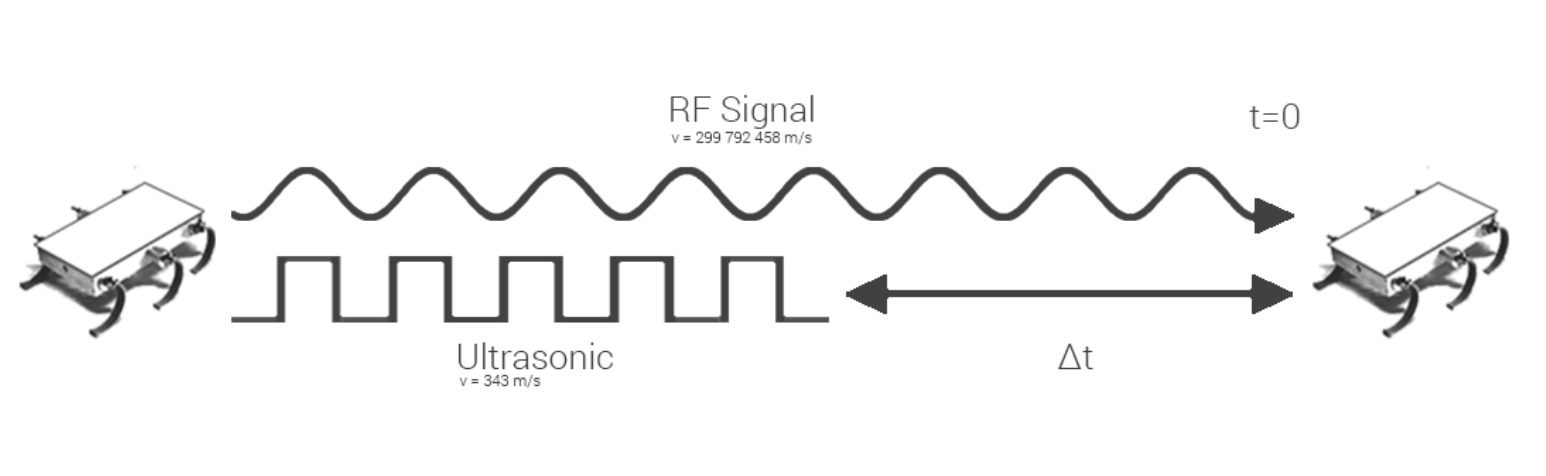
\includegraphics[width=0.8\textwidth]{Figures/Rf_vs_Us.jpeg}
\caption{TDOA of RF message and ultrasonic pulse}\label{fig:ultra1}
\end{figure}

Because the range of the RF message is easily 3 times the range of the ultrasonic pulse, which can be further limited by the receiving circuit, a Zebro will never receive an ultrasonic pulse without the accompanying RF message. Furthermore the RF message is hopped trough the Zebro swarm making sure that the message reaches all Zebros.

\begin{figure}[H]
\centering
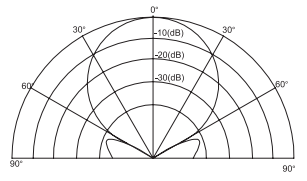
\includegraphics[width=0.5\textwidth]{Figures/ultrasonics_transceivers.PNG}
\caption{Directivity of an ultrasonics transducer}\label{fig:ultra2}
\end{figure}

%----------------------------------------------------------------------------------------
%	Tade-off
%----------------------------------------------------------------------------------------

\section{Concept implementations}
In this section we're going to look at the options to implement the concept. A comparison between the different options is made, where necessary with a criteria trade-off. Furthermore we will discuss the options for the implementation of the ultrasonic transducers, the transmitter circuit and the receiver circuit.

\subsection{Ultrasonic transducers}

One problem arises: Ultrasonic transducers don't send omnidirectional, they have a narrow beam width.
Most available transducers have a beam angle of \SI{50}{\degree} to \SI{80}{\degree}, far from the \SI{360}{\degree} we need to comply to requirement~\ref{req:omnidir}.
Two possible solutions are considered: using multiple transducers to implement a \SI{360}{\degree} transducer array or creating a omnidirectional antenna to shape the directivity of a single transducer.

We make the design trade-off based on a set of design criteria: cost, power consumption, size, precision, angle of arrival (AOA) measurements.
A system using multiple transducers would need between 4 to 8 sensors to create an omnidirectional array while the antenna systems needs a single transceiver.

\begin{table}[H]
\centering
\begin{tabular}{|l|c|c|}
    \hline
    Criteria            & Omnidirectional   & Sensor array \\
    \hline
    Cost                & ++ & -  \\
    Power consumption   & + & - \\
    Size                & - & - \\
    Range               & - & + \\
    Accuracy            & - & - \\
    AOA detection       & - & (+) \\
    \hline
\end{tabular}
\caption{Criteria comparison}
\label{tab:ant_crit}
\end{table}


\begin{itemize}
    \item
      \textbf{Cost:} The estimated cost of an ultrasonic transceiver is \euro{3} for a \SI{50}{\degree} beam width model and \euro{5} for a \SI{80}{\degree} beam width model.
      For the antenna the entire beam has to be incident on the lens of the antenna so a sensor with a small beam width (focused on the lens) is preferred.
      The antenna system needs a single transceiver since the antenna can both transmit and receive ultrasonic waves.
      The production cost of the 3D printed antenna is estimated at \euro{2}.
      The total cost would be \euro{5} plus the cost of a driver and receiver circuit.
      For the array we need at least 4 times the \SI{80}{\degree} sensors or 7 times the \SI{50}{\degree} sensors costing roughly \euro{20}.
      Furthermore we need an structure to hold the sensors at the correct angles an multiple versions of the driver and receiver circuit increasing the cost. This means the antenna systems is roughly a fifth of the price of the sensor array.
    \item
      \textbf{Power consumption:} The array would use x times the power of the antenna system where x is the number of sensors in the array.
    \item
      \textbf{Size:} The antenna system would need an exterior reflecting located on top of the system while the array systems needs more space on the circuit board, since it uses multiple drive and receiver circuits, increasing the internal space needed to house the electronics.
      Since the module is located on top of the Zebro an increase in required internal space requires a higher module so we assume that the space needed for both systems is roughly the same.
    \item
      \textbf{Range:} Since the array uses a direct configuration the received power will be higher than that off the antenna system where the waves are reflected by the lens.
      The traversed path with the antenna system is longer since the waves have to travel the extra distance to the lens and the waves are reflected in a \SI{360}{degree} pattern so that a large part of the power does not arrive at the receiver.
    \item
      \textbf{Accuracy:} We assume that there is no accuracy difference between the two systems since both only transmit a short ultrasonic pulse.
      If the ultra sonic signal would have contained information this would be distorted by the reflecting antenna.
      The only difference we expect is a time offset resulting from the extra distance the ultra sonic pulse has to travel in the antenna system. This offset is constant so easily compensated.
    \item
      \textbf{AOA detection:} An array of ultrasonic sensors gives us the possibility of calculating the AOA by comparing the difference in TOA or received power of the different sensors.
      We can estimate the same angle with the correct filter technique, as discussed in \cite{processing}, this makes the AOA capabilities of the array redundant.
\end{itemize}

Based on the criteria comparison we choose to design a distance sensing system which uses an antenna to create an omnidirectional beam pattern. This system uses a single ultrasonic transducer which can act as both a transmitter and receiver. To operate this transducer we need a switching circuit which allows us to select transmitter or receiver mode. In transmitter mode the microcontroller will generate a PWM pulse at 0-5V. This PWM pulse is amplified to generate the pulse necessary to drive the ultrasonic transducer. In receiver mode the signal detected by sensor is first amplified and then processed by a detector circuit. This detector circuit will give a high output when no signal is detected and a low output when the sensor detects a signal. The microcontroller can detect the change from high to low to determine when the ultrasonic pulse is received. The detector signal is high when there is no signal so that the system can check if the receiver section is working properly. When the systems switches to receiving mode but doesn't detect a high detection signal the microcontroller knows that there is a problem in the receiver section. An overview of this concept is given in figure ~\ref{fig:ultra3}. In the next subsections we will discuss the possible implementations of the required transmitter and receiver circuit.

\begin{figure}[H]
\centering
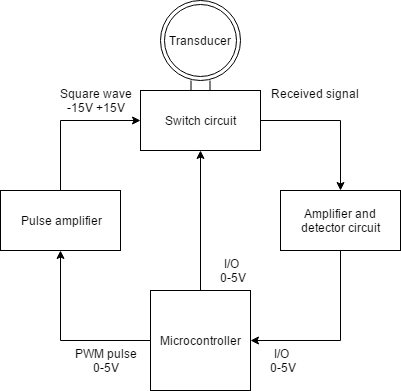
\includegraphics[width=0.6\textwidth]{Figures/concept.png}
\caption{Block diagram of distance sensing system}
\label{fig:ultra3}
\end{figure}

\subsection{Transmitter}
\label{chap:trans}

To transmit a ultrasonic signal the transducer needs to be driven by a \SI{40}{\kilo\hertz} wave.
Typical voltage levels for this wave are between $5V_{p-p}$ and $40V_{p-p}$ and is symmetrical around 0 ($V^{+}=-V^{-}=\frac{1}{2}V_{p-p}$).
We discuss 2 options to generate the \SI{40}{\kilo\hertz} \SI{50}{\percent} duty cycle wave: an operational amplifier circuit and a H-bridge driver circuit.

The operational amplifier circuit uses a comparator with supply voltage ($V^{+}=\frac{1}{2}V_{p-p}$) and ($V^{-}=-\frac{1}{2}V_{p-p}$).
When the input signal of the comparator, a \SI{50}{\percent} PWM generated by the micro controller, is above a certain threshold $V_{th}$ the output is $V^{+}$.
When the input is below $V_{th}$ the output of the comparator is $V^{-}$.
The threshold is set at half the amplitude of the PWM generated by the micro controller (typical 5V).
Since the battery output is a positive voltage \ref{req:volt} we need to create the negative supply voltage inside the module.
MIT uses an IC in their ultrasonic transmitter driver circuit that converts the VCC power supply to an $V^{+}$ and a $V^{-}$ to power the operational amplifier.
However, this IC is relatively expensive in SMD design package.

H-bridge driver circuits are typically used for motor driving circuits but, with the right selection of components, can be adapted to drive a ultrasonic transducer.
The H-bridge switches the polarity off the voltage on the ultrasonic transducer generating a PWM driving signal.
The amplitude of this signal is the supply voltage of the H-bridge.
The circuit does not require a negative supply voltage but needs 2 control waveforms which are the logic inverse of each other.
These control waveforms need to be generated by the micro controller directly or trough an inverter circuit.

Since we are not sure which solution will give the best transmitting results, we will test both circuit solutions. The first solution, the op-amp circuit, is relatively expensive because of the voltage converter, but we are sure this will work because it is already proofed on with the Cricket circuit. The H-bridge driver is typically used to drive motors so we are not sure if this will also work to drive ultrasonic transceivers. The results of H-bridge circuit will be discussed in section \ref{sec:transcircuit}.

\subsection{Receiver}
\label{chap:receiver}

The receiver circuit needs to detect if an ultrasonic signal is present.
When it receives an ultrasonic pulse it's output ($US_{detect}$) will go low allowing the microcontroller to determine at which point in time the pulse reached the ultrasonic transducer.
The MIT Cricket indoor location system \cite{Balakrishnan2003, Priyantha2000} project has used two types of detection circuits: A phase-locked loop (PLL) in combination with a tone detector and as a second option an amplitude detection circuit.
Before the detector circuits are able to detect an ultrasonic pulse the received signal needs to be amplified.

The PLL detector generates a output signal whose phase is related to the phase of the input signal.
This means that the frequency of the output signal is the same as the frequency of the input signal.
Since the frequency of the ultrasonic pulse is known to be \SI{40}{\kilo\hertz}
the signal can be recovered from the ultrasonic transducer.
The output of the PLL will then be a signal with a frequency of \SI{40}{\kilo\hertz} when the transducer receives an ultrasonic pulse.
The signal will then be presented to a tone detector which detects if the signal has a frequency of \SI{40}{\kilo\hertz} or not.
The output of this tone detector is high when the frequency of it's input is not \SI{40}{\kilo\hertz}, which corresponds to not receiving an ultrasonic pulse, and low when the frequency of it's input is \SI{40}{\kilo\hertz} corresponding to receiving an ultrasonic pulse.

The second solution, the amplitude detector, uses a peak detection circuit to detect the amplified received signal.
The peak detection circuit consists of a diode, a capacitor and a resistor as pictured in \ref{fig:peak_d}.
The signal on the input of the detector charges the capacitor.
When the ultrasonic transducer doesn't receive a signal the amplified received signal will be a DC voltage.
In this case the output of the detector circuit will be the input DC voltage.
When the transducer does receive an ultrasonic signal the input will be a biased sinusoidal wave.
The bias of this sinusoidal wave is the DC voltage present when the systems doesn't receive an ultrasonic signal.
Now the capacitor is charged by the sinusoidal wave and discharges over the resistor.
The capacitor charges due to this sinusoidal wave, the voltage over the capacitor basically follows the input voltage source.
It will charge up to the peak voltage of the signal. Once it reaches this voltage, the capacitor discharges over the resistor.
It does not discharge back through the diode because the diode is a one-way current device.

The voltage across the capacitor isn't directly the peak voltage of the waveform.
This is because the diode consumes some voltage.
Therefore the maximum voltage measured across the output is actually higher than the input voltage by a factor of the voltage drop across the diode.
To get the true peak voltage, we must subtract the voltage that the diode consumes from the output signal.
So if we measure the voltage at the capacitor to be 9V and the diode consumes 0.6V, the peak voltage of the input signal is actually \SI{8.4}{\volt}.

The time it will take for the capacitor to completely discharge is 5RC, where R is the resistance and C is the capacitance.
This time needs to be larger than the time of a half period of the 40 kHz signal, which is 0.0125 $ms^{-1}$.
So the RC need to be larger than $5 * 0,0125 ms^{-1} = 0.0625ms^{-1}$.
With this RC the capacitor discharges slowly enough to have a signal so the comparator can detect the difference between a received and not received signal.\footnote{The final values differ from the given RC value. This is due the non ideal behaviour of physical capacitors. The final values as given in the circuit of appendix \ref{Appendixcircuits} are found by testing different configurations.}

\begin{figure}[H]
\centering
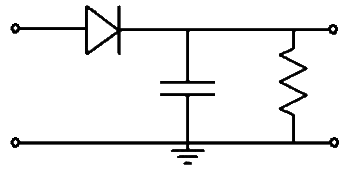
\includegraphics[width=0.4\textwidth]{Figures/peak_d.PNG}
\caption{Peak detection circuit}
\label{fig:peak_d}
\end{figure}

The first version of the MIT Cricket indoor localisation system used a PLL to detect the ultrasonic signal \cite{Priyantha2000}.
In \cite{Balakrishnan2003} the lessons learned from Cricket V1 and explain that the PLL system had highly variable detection characteristics leading to high measurement errors.
They have since then implemented a amplitude detection circuit and found it to improve detection accuracy.
Using this knowledge we opt to design our own peak detection system instead of a PLL.

\section{Antenna design}
The first thing that is considered is the shape of the ultrasonic reflecting antenna. An optimised design is not in the scope of this projects so we will be basing our design on three basic antenna shapes: cone, sphere and parabolic.

\begin{figure}[H]
\centering
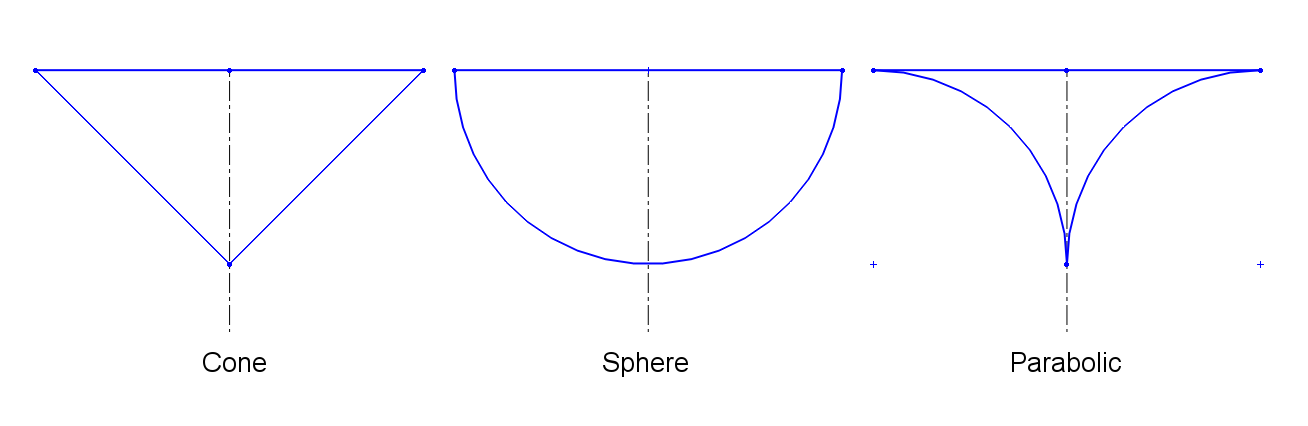
\includegraphics[width=0.9\textwidth]{Figures/ant_shapes.PNG}
\caption{Possible shapes for the reflector antenna, the cone, the sphere and the parabolic design}
\label{fig:shapes}
\end{figure}

Requirements for the antenna are is:

\begin{enumerate}[label={[A.\arabic*]}]
  \item
  \textbf{Transmitting and receiving:} The antenna should be usable in both a transmitting and a receiving configuration. All robots will be fitted with the same antenna and will be using a single ultrasonic transducer. \label{ref:T_R}
  \item\label{ref:a2}
  \textbf{Lightweight:} The antenna should be lightweight because it will be mounted on top op the Zebro. For stability a low centre of mass favourable.
  \item\label{ref:a3}
  \textbf{Mass production:} It has to be possible to produce the final design in large quantities.
  \item
  \textbf{Stable:} Movement of the Zebro should not change the transmitting/receiving behaviour due to movement of components in the antenna.
\end{enumerate}

To comply to requirement \ref{ref:a2} and \ref{ref:a3} we decide to produce the antenna from plastic. It's lightweight, can be produced an mass by making moulds and reflects ultrasonic waves.
The prototype will be 3D printed since the initial costs for making a mould are high and the prototype series will consist of only 5 antennas.

An numerical design for such an antenna is not in the scope of this project so we will use a wave reflection simulation tool to select the most suitable antenna shape.
Figure~\ref{fig:shapes} shows the antenna shapes we will simulate.
The figure shows half of the shape where the dotted line is the central axis of the reflector antenna.
The ultrasonic transducer will be centred on the central axis of the antenna below the reflecting surface such that the system is symmetrical.

After the simulations we will design a proof of concept version of the selected antenna.
The design of this proof of concept antenna is discussed in section ~\ref{sec:antenna_proof}.

\section{Transmitter circuit design}
\label{sec:transcircuit}

For the design of the transmitter circuit, there are two possible solutions as discussed in section \ref{chap:trans}. The first solution is the operational amplifier circuit, and the second solution is the H-bridge driver circuit.

The idea for the operational amplifier circuit is from the MIT ultrasonic transmitter driver circuit \cite{Priyantha2005}. MIT uses an IC that converts the VCC power supply to an $V^{+}$ and a $V^{-}$ to power the operational amplifier. However, this IC is relatively expensive in SMD design package. The circuit is simple because it can be driven directly out of an I/O pin of the micro controller. The signal out of the micro controller is than compared to a DC value, $V_{th}$, set on the negative pin of the operational amplifier. In this configuration the operational amplifier works as a comparator. A value on the plus pin above $V_{th}$ results in an output of $V^{+}$ and a value underneath $V_{th}$ result is an output of $V^{-}$. If the op-amp is driven with a PWM with duty cycle of 50\% and a $V_{th}$ of $\frac{1}{2}V_{p-p}$ of the I/O pin, the output of the op-amp will be symmetrical around 0 and have a wave with amplitude of $2 * V^{+}$. These outputs are desired to drive the ultrasonic transceiver.

In figure \ref{fig:h_bridge} is a typical H-bridge circuit visible. The ultrasonic transceiver is placed over the connectors J1 and J2. If signal S1 is high, J1 is connected to $VCC$ and if S2 is low, J2 will be connected to ground. Let's say this is the forward mode. The reverse mode is when S2 is high and S1 is low, than J1 is connected to ground and J2 is connected to $VCC$. In this way the ultrasonic transceiver is driven with a $V_{p-p}$ of $2 * VCC$ using only one positive power source. The output signal over J1 and J2 is symmetrical around 0 if S1 and S2 are driven with a PWM with a duty cycle of 50\%. This are, again, the desired outputs to drive the ultrasonic transceiver. The H-bridge solution seems more legit since it only uses one $VCC$ power source and no voltage converter IC in front.

\begin{figure}[H]
\centering
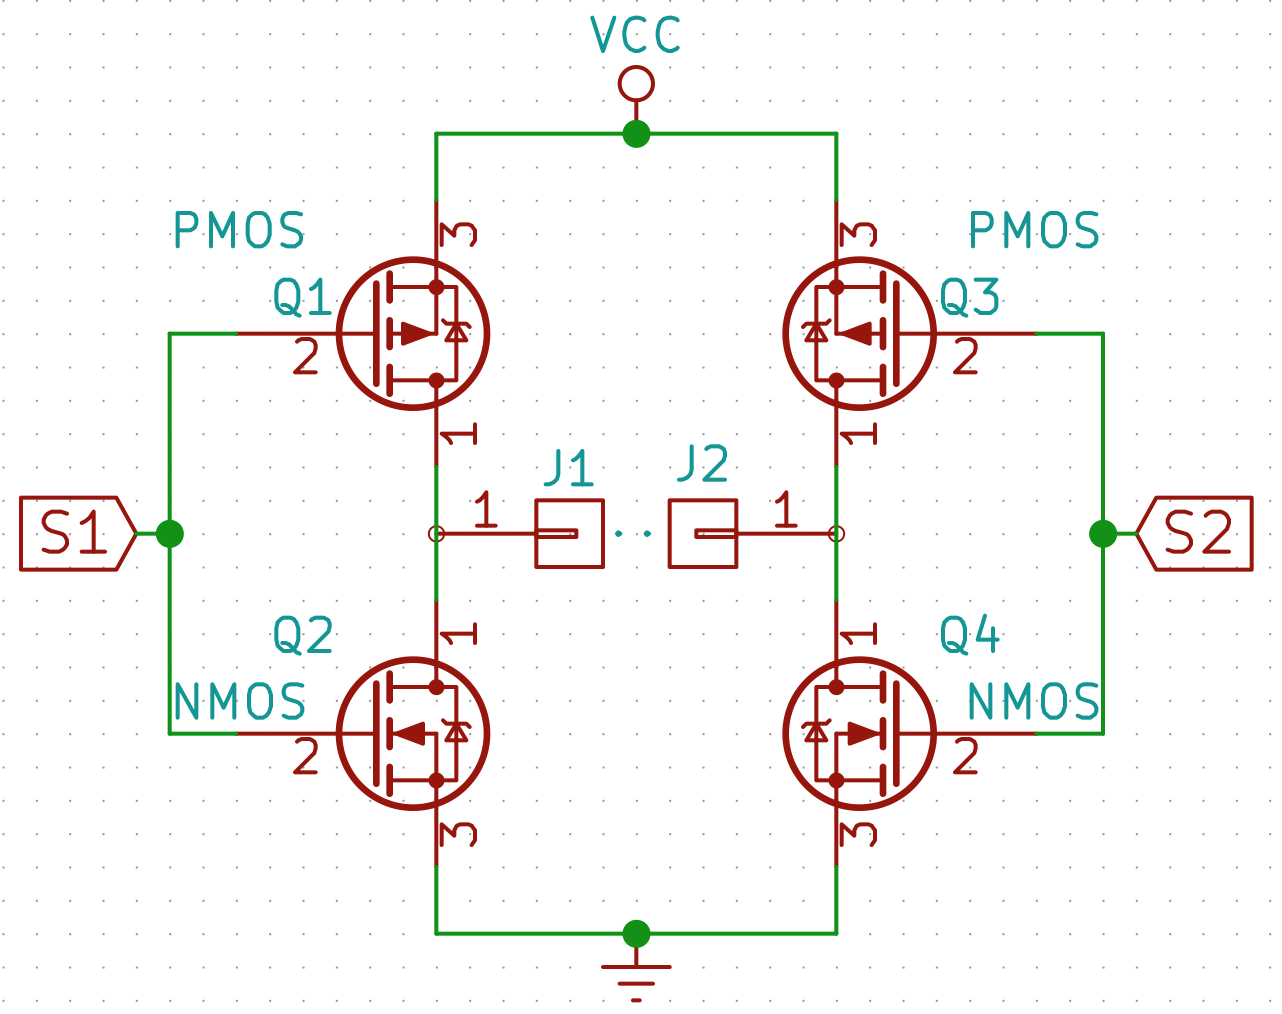
\includegraphics[width=0.6\textwidth]{Figures/hbridge.PNG}
\caption{H-bridge circuit}
\label{fig:h_bridge}
\end{figure}

To get a 30 $V_{p-p}$ PWM signal, with frequency of 40 kHZ, on the ultrasonic transceiver the $VCC$ needs to be 15V. But if the $VCC$ is 15V the MOSFET's can't be turned on and off directly out of the I/O pins of the micro controller. This is why the H-bridge needs to have a high side driver circuit, or IC, in front. After all we found an IC, the MIC4428 \cite{MIC4428}, that has typical applications to drive piezoelectric transducers and have a driver and H-bridge circuit integrated.

\section{Receiver circuit design}
\label{chap:receivercircuit}
For the receiver circuit design there were two types of detection circuits discussed before in section \ref{chap:receiver}. But regarding the conclusions of Cricket V1 we chose to use the peak detection circuit in stead of the phase lock loop detector circuit.

The ultrasonic transceiver can receive 40 kHz signals, also known as ultrasonic signal. These received signals have a very low amplitude, this is why the detection circuit needs to have an amplification. The amplification can be done using an operational amplifier. Literature study showed that one stage amplification gives a to low amplification, this is why we use a two stage operational amplification. As can be seen in figure \ref{fig:receivecircuit} the op-amps U2A and U2B are the two stages for the amplification.
The ultrasonic transceiver is connected to 1Y1 and 1Y2, as can be seen in in the figure \ref{fig:receivecircuit}. The ultrasonic transceiver is biased at a voltage of half the supply voltage of the first two stages, in this design it is $4.5V$, since we power the op-amps with $9V$. This is because the signal received on the ultrasonic transceivers is symmetrical around 0 which holds that is also receives negative voltages, but since we only power the op-amps with a positive voltage and ground we biased the ultrasonic transceiver. In this way we amplify both the positive and negative received amplitudes of the signals.
%The configuration in which the first two stages are used is called the differential amplifier configuration.
In the feedback loops of the op-amps are pot meters visible, this is to tune the amplification of both op-amp stages.\footnote{The final values of the feedback resistors are given in the circuit of appendix \ref{Appendixcircuits}.}

\begin{figure}[H]
\centering
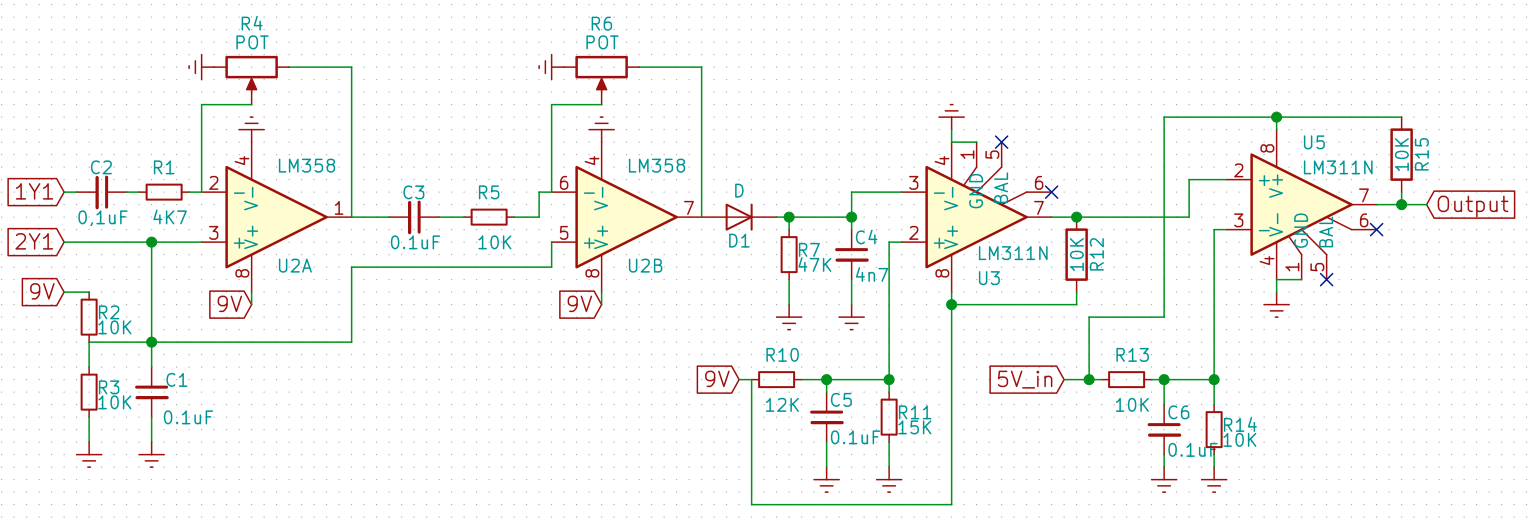
\includegraphics[width=0.9\textwidth]{Figures/receivercircuit.PNG}
\caption{The receiver circuit for the ultrasonic transceiver}
\label{fig:receivecircuit}
\end{figure}

A simple simulation that visualises what happens when the ultrasonic transceiver is not biased is visible in figure \ref{fig:nonbias}.
And a simulation where the ultrasonic transceiver is biased by half the power of the op-amp is visible in figure \ref{fig:bias}
We can conclude form these figures that it is better to bias the transceiver if we only power the operational amplifiers with a positive voltage and ground. Because with the non biased configuration, half of the signal information is thrown away.

\begin{figure}[H]
\centering
\begin{subfigure}{.5\textwidth}
  \centering
  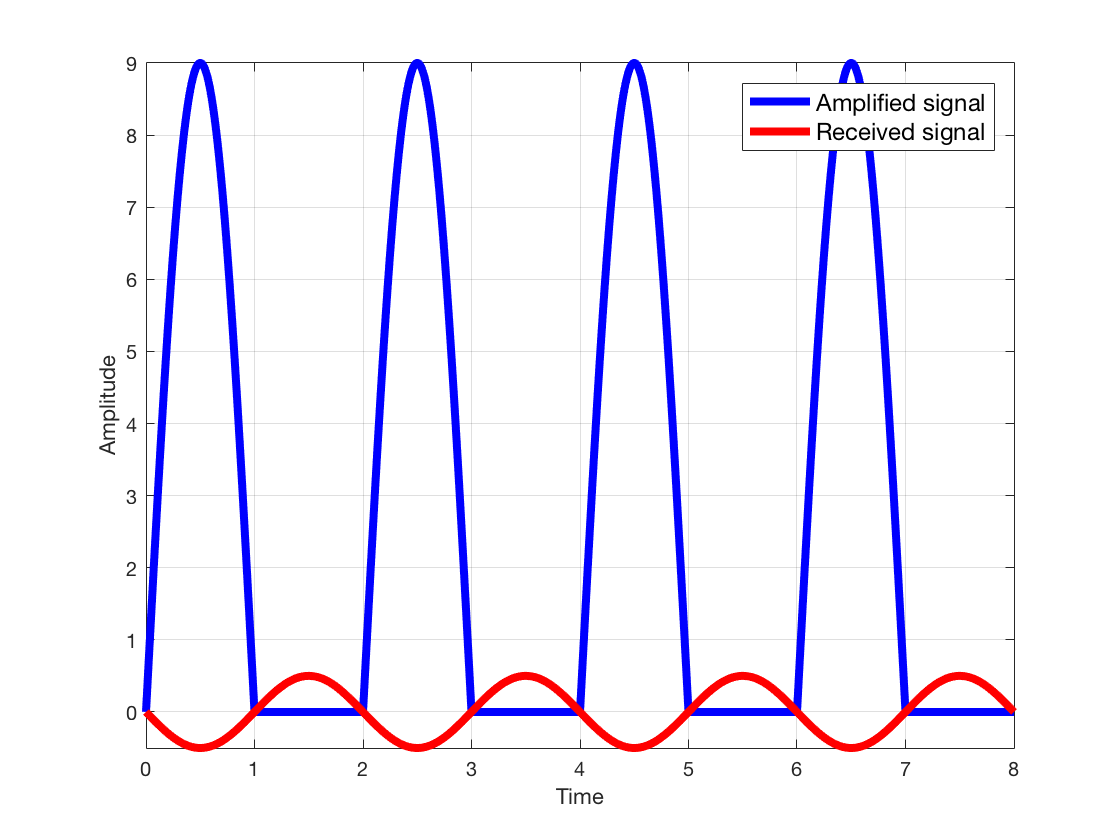
\includegraphics[width=1.0\textwidth]{Figures/nonbias.PNG}
  \caption{A simultion with no bias voltage}
  \label{fig:nonbias}
\end{subfigure}%
\begin{subfigure}{.5\textwidth}
  \centering
  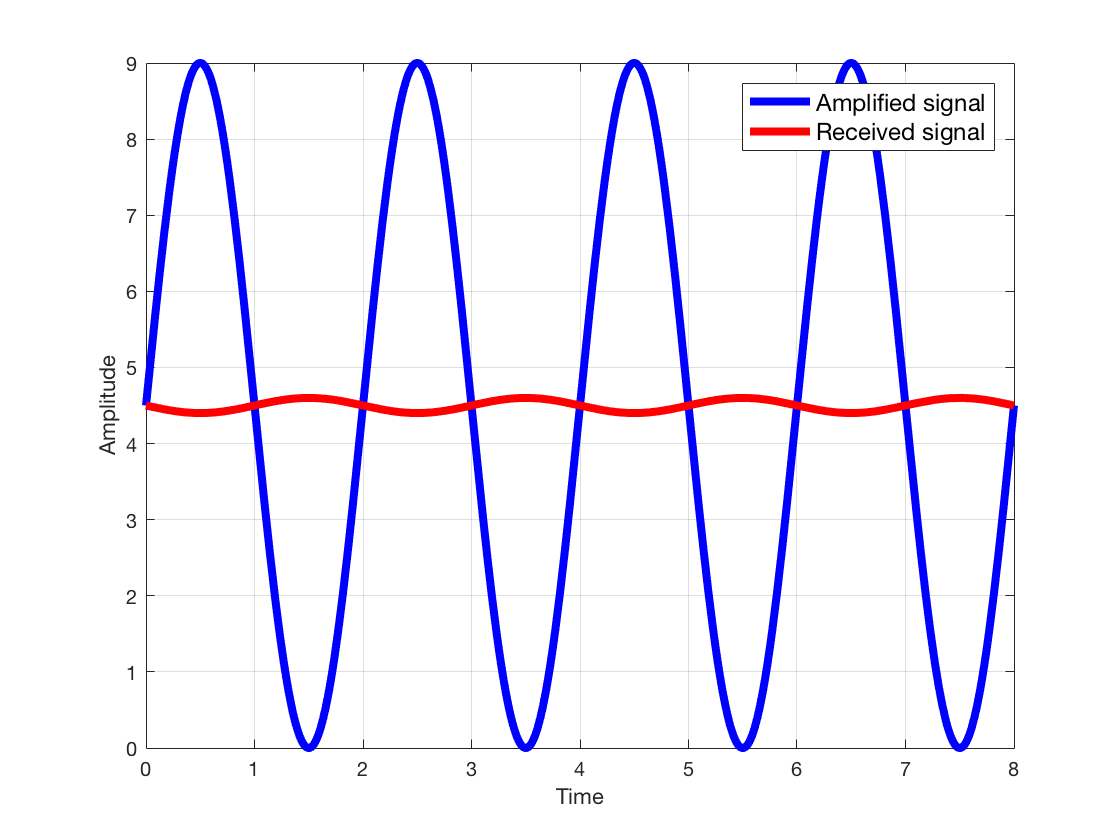
\includegraphics[width=1.0\textwidth]{Figures/bias.PNG}
  \caption{A simultion with bias voltage}
  \label{fig:bias}
\end{subfigure}
\caption{Bias simulations for the ultrasonic transceiver}
\label{fig:simulationsbias}
\end{figure}

After the two stages of amplification, the peak detection circuit is visible in figure \ref{fig:receivecircuit}. The peak detection circuit consists of a diode D1, a resistor R7 and a capacitor C4. The peak detection circuit is already mentioned before in section \ref{chap:receiver}. The desired output of the peak detection is visible in figure \ref{fig:waves_peak_detect} as the V receiving signal, the signal when not receiving an ultrasonic signal is $4.5V$ since the + pin of the op-amps of the first and second stages are kept at $4.5V$.
After the peak detection circuit, a comparator is visible in figure \ref{fig:receivecircuit}. This comparator compares the signal on the - pin of U3 to the DC value, $V_{th}$, put on the + pin of U3. This $V_{th}$ needs to be chosen to sit in between the value of the not receiving voltage and the minimum value of the receiving signal voltage on the input of the comparator, this is visible in figure \ref{fig:waves_peak_detect}. The comparator is in the circuit because we want to detect a falling edge when the ultrasonic transceiver receives a ultrasonic pulse.

The last comparator stage in the circuit makes the signal output an output that is between the desired voltages for the micro controller, 0 and 5 volt. Directly powering the first comparator stage of U3 with $5V$ could also result in an output between 0 and 5 volt, but since the $V_{th}$ is close to the supply voltage of the comparator is this not allowed.

In the rest of the circuit are some stabilisation capacitors visible to stabilise the voltages put on several pins. The capacitors C2 and C3 give the operational amplifiers an active high pass filter. The cut off frequency can be calculated with equation \ref{eq:cutof}
The first stage cut off frequency is 338.6 Hz and the cut off frequency of stage two is 159.2 Hz
\begin{equation}
\label{eq:cutof}
F_{c}= \frac{1}{2\pi RC}
\end{equation}

\begin{figure}[H]
\centering
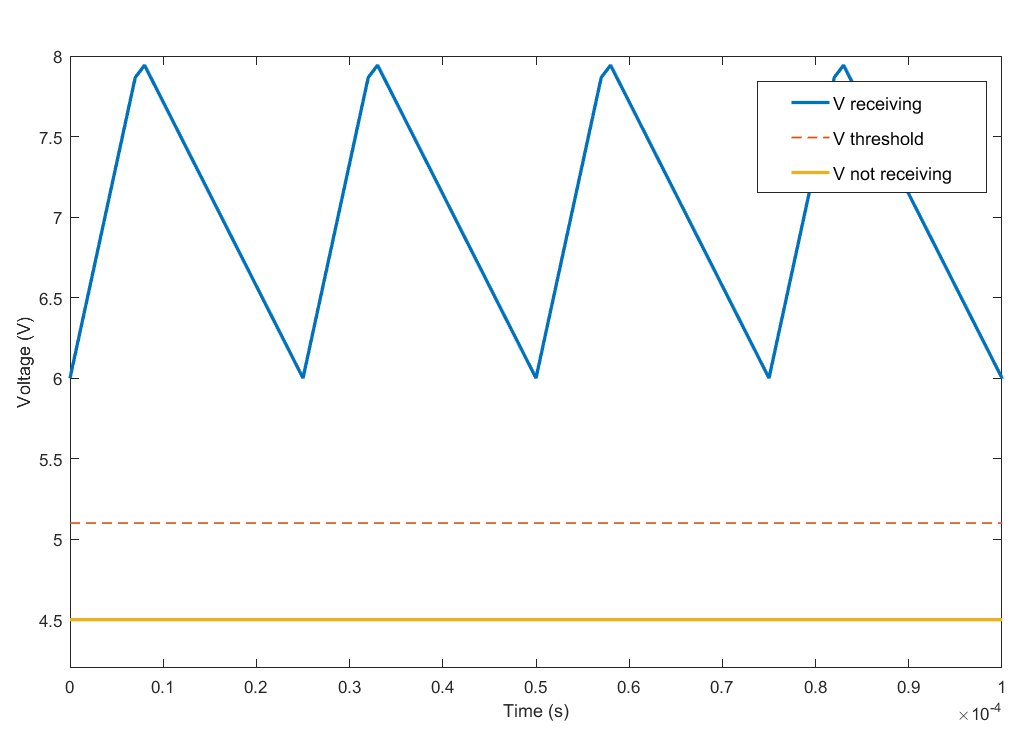
\includegraphics[width=0.85\textwidth]{Figures/waves_peak_detect.png}
\caption{Desired output peak detect circuit}
\label{fig:waves_peak_detect}
\end{figure}

\section{Simulations}

\subsection{Antenna}

Using an simulation tool \cite{Ultratool} we were able to simulate the different antenna lens shapes.
The tool is originally designed for optics but it's suitable to simulate the far field behaviour of sound waves.
Below the results of the simulations are given and discussed.
We will first look at the transmitting behaviour of the different shapes.
The most suitable shape for our application is selected.
Last we simulate the receiving behaviour of the selected shape to see if we comply to requirement \ref{ref:T_R}.

For the simulation we simulated the ultrasonic transducer by placing a point source in an enclosure such that we get a beam width of \SI{50}{\degree}.
The reflecting surface is then placed above the simulated transducer.
Figures~\ref{fig:sim_cone_45}-\ref{fig:sim_para} show the right half of the symmetrical simulation results.
The ultrasonic transducer, simulated by a point charge, is located at the red dot lying beneath the reflecting surface.

\begin{figure}[H]
\centering
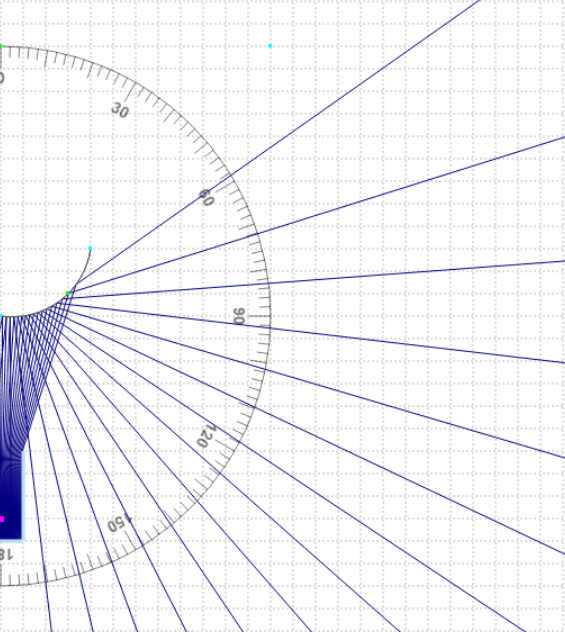
\includegraphics[width=0.6\textwidth]{Figures/sim_globe.PNG}
\caption{Simulation of transmitting with a globe shaped lens}
\label{fig:sim_globe}
\end{figure}

The spherical shaped lens in figure~\ref{fig:sim_globe} scatters the waves in a wide spread pattern.
The energy transmitted at an angle, with respect to the transmitter axis, greater than \SI{120}{\degree} does not reach the other Zebros.
This means a large part of the generated energy is lost as it's transmitted towards the Zebro body and not to the antenna of the other Zebros.
In conclusion the sphere produces an unfocussed radiation pattern.

\begin{figure}[H]
\centering
\begin{subfigure}{.5\textwidth}
  \centering
  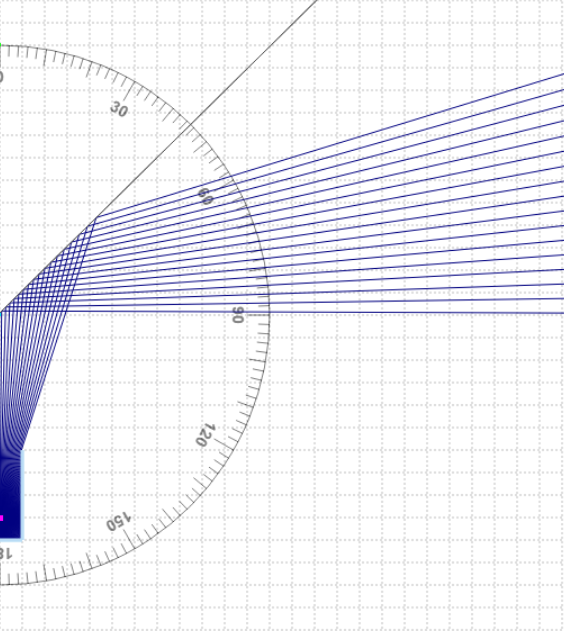
\includegraphics[width=0.85\textwidth]{Figures/sim_cone_45.PNG}
  \caption{45 degree cone}
  \label{fig:sim_cone_45}
\end{subfigure}%
\begin{subfigure}{.5\textwidth}
  \centering
  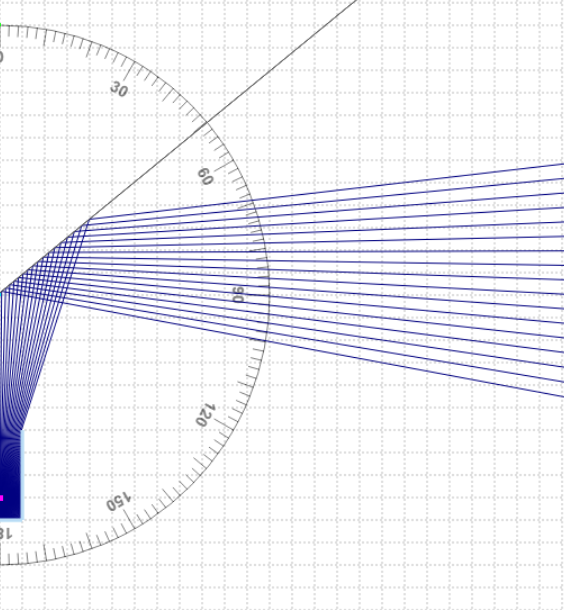
\includegraphics[width=0.9\textwidth]{Figures/sim_cone_50.PNG}
  \caption{50 degree cone}
  \label{fig:sim_cone_50}
\end{subfigure}
\caption{Simulation of transmitting with a cone shaped lens}
\label{fig:cone}
\end{figure}

%\begin{figure}[H]
%\centering
%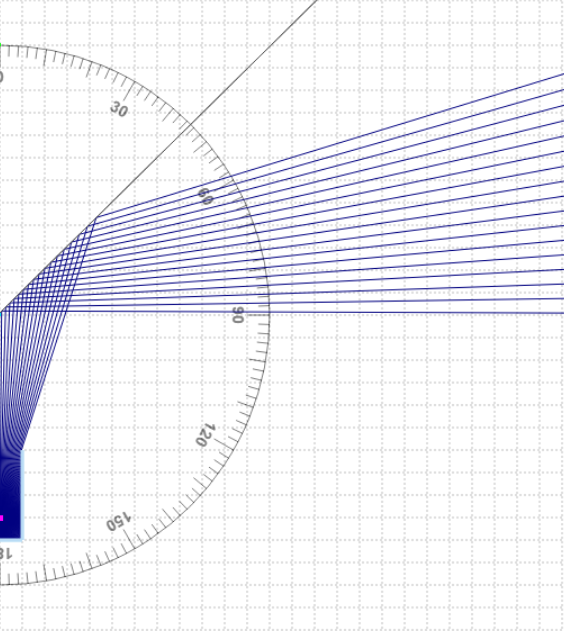
\includegraphics[width=0.6\textwidth]{Figures/sim_cone_45.PNG}
%\caption{Simulation of transmitting with a 45 degree cone shaped lens}
%\label{fig:sim_cone_45}
%\end{figure}

We see from figure~\ref{fig:sim_cone_45} that the cone produces a focussed beam.
In this case the beam is focused around \SI{75}{\degree} meaning that the energy is directed upwards instead of in the horizontal direction.

%\begin{figure}[H]
%\centering
%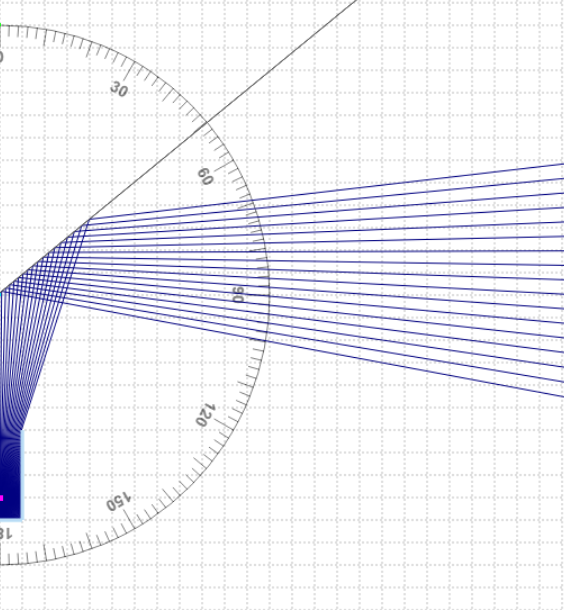
\includegraphics[width=0.6\textwidth]{Figures/sim_cone_50.PNG}
%\caption{Simulation of transmitting with a 50 degree shaped lens}
%\label{fig:sim_cone_50}
%\end{figure}

The \SI{50}{\degree} cone produces a beam focused around \SI{90}{\degree} as seen in figure~\ref{fig:sim_cone_50}.
In this case the energy is directed in the horizontal direction.

\begin{figure}[H]
\centering
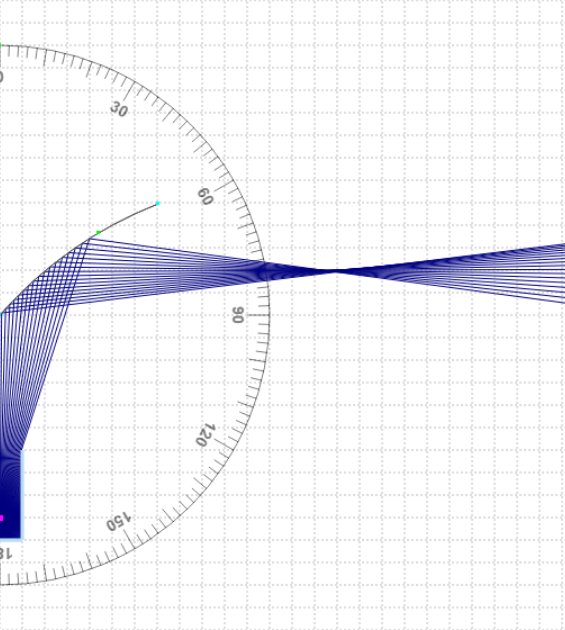
\includegraphics[width=0.6\textwidth]{Figures/sim_par.PNG}
\caption{Simulation of transmitting with a parabolic shaped lens}
\label{fig:sim_para}
\end{figure}

The parabolic antenna allows us the set a focal point for the beam as seen in figure~\ref{fig:sim_para}.
This would be ideal if the distance between Zebros is static so we could place the focal point on the antenna of the other Zebros.
In a moving swarm this Antenna has no advantage over the other shapes.

Comparing the simulation results shows us that for our situation, moving robots in the horizontal plane, the \SI{50}{\degree} cone antenna is the best option.

\begin{figure}[H]
\centering
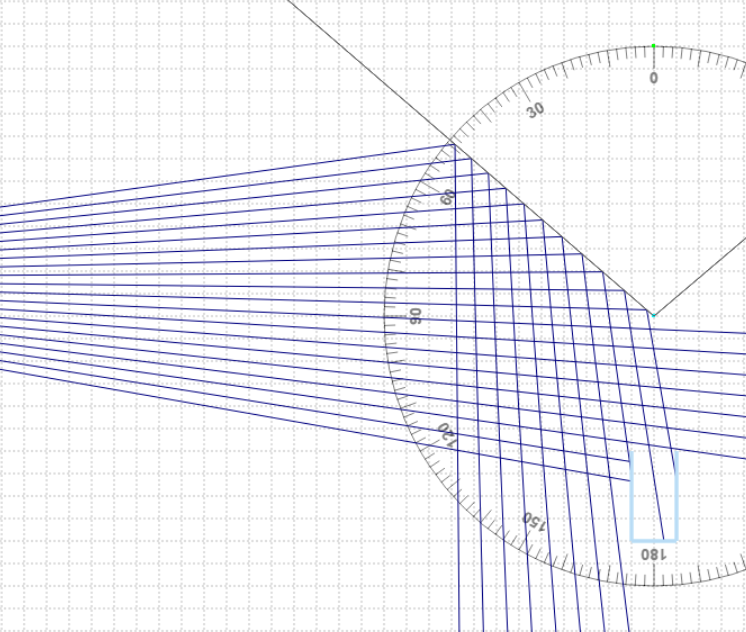
\includegraphics[width=0.6\textwidth]{Figures/sim_cone_rec.PNG}
\caption{Simulation of receiving with a \SI{50}{\degree} cone shaped lens}
\label{fig:sim_cone_rec}
\end{figure}

Figure~\ref{fig:sim_cone_rec} shows the receiving behaviour of the \SI{50}{\degree} cone when waves, reflected by another \SI{50}{\degree} antenna, are incident on the lens.
We see that the incident waves are reflected towards the transducer at the centre of the lens.
This means that the \SI{50}{\degree} antenna is both suitable for transmitting and receiving the ultrasonic pulse.

\subsection{Receiver circuit simulations}

In figure \ref{fig:sim_receive} and \ref{fig:sim_receive2} are Falstad \cite{Falstad}
simulations visible of the receiver circuit discussed before in section \ref{chap:receivercircuit}. In the figure are 4 signals visible:

\begin{itemize}
\item
The green signal, the signal after the first stage of amplification
\item
The red signal, the signal after the second stage of amplification
\item
The orange signal, the signal after the peak detection circuit
\item
The pink signal, the $V_{th}$ of the first comparator stage
\end{itemize}

Figure \ref{fig:sim_receive} shows the operation amplifier signals of the receiver circuit. Between 0 and $0.075*10^{-1}ms^{-1}$ no ultrasonic signal is detected on the transceiver, between $0.075*10^{-1}$ and $0.525*10^{-1}ms^{-1}$ the ultrasonic transceiver receives a ultrasonic signal. And after $0.525*10^{-1}ms^{-1}$ the ultrasonic transceiver receives no ultrasonic pulse any more.
The signal received on the ultrasonic transceivers have an amplitude between the 0 and $100mV$. This signal is amplified in the first stage of the circuit, this is the green signal in figure \ref{fig:sim_receive}. The second stage amplification results in a signal with a higher amplitude, with a maximum amplitude of $4.5V$ due to the $4.5V$ put on the plus pin of the operational amplifier and the power source of $9V$. This signal is visible in the figure as the red signal.
The peak detection circuit charges a capacitor in this circuit, and discharges over a resistor. This results in the orange signal. This makes it possible to detect if there is an ultrasonic signal received. If the voltage of the peak detection signal is higher than the $V_{th}$, the pink signal, the comparator switches it's output. And if the peak detection signal becomes lower than the $V_{th}$ the comparator signal switches back. Both happen with a bit of delay since the capacitor needs to be charged or discharged. So the desired signal of the peak detection circuit needs to rise and fall fast, but not too fast otherwise the peak detection circuit won't work any more.\\

\begin{figure}[H]
\centering
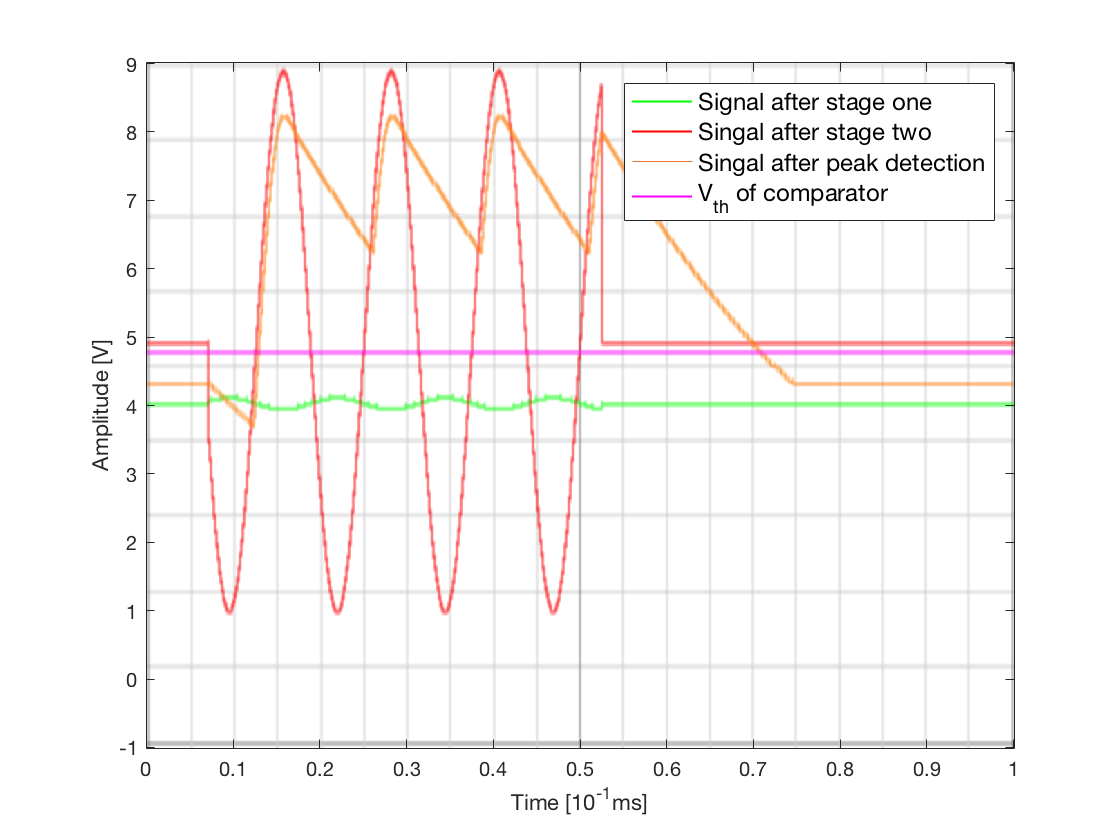
\includegraphics[width=0.85\textwidth]{Figures/receiver_simulations.PNG}
\caption{Simulation of receiver circuit, operational amplifier signals}
\label{fig:sim_receive}
\end{figure}

\begin{figure}[H]
\centering
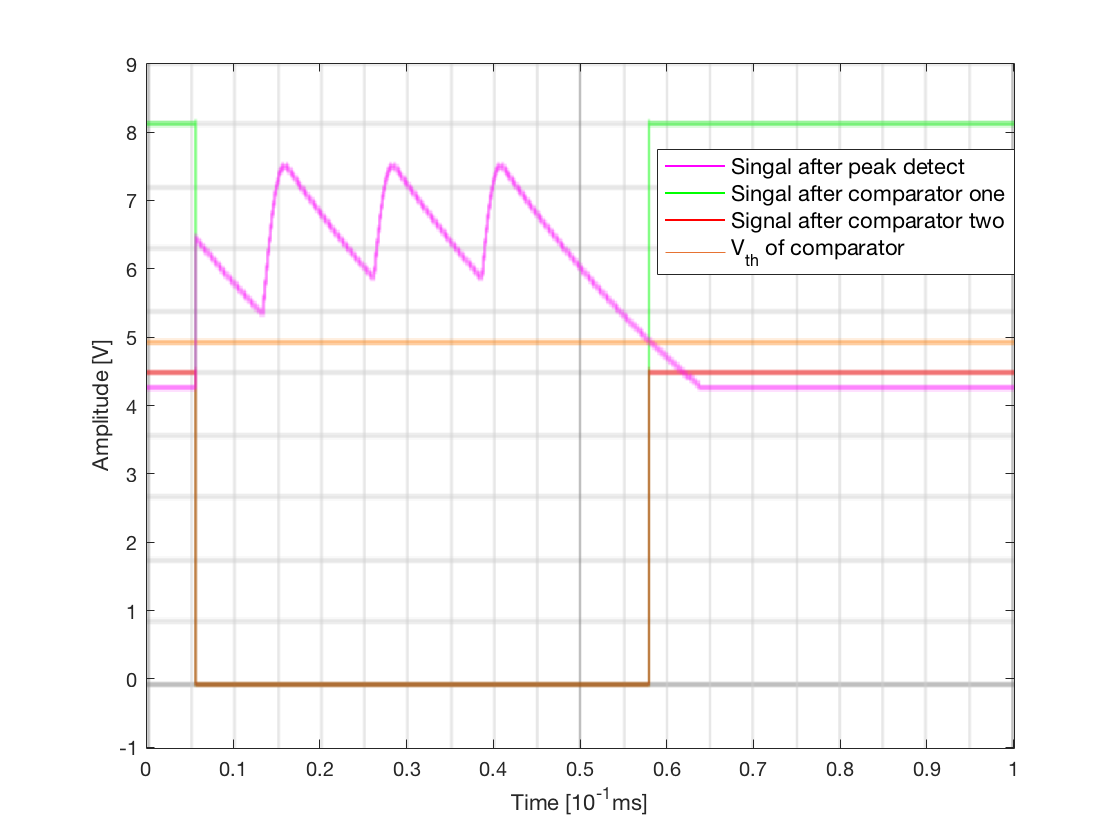
\includegraphics[width=0.85\textwidth]{Figures/receiver_simulations2.PNG}
\caption{Simulation of receiver circuit, comparator signal}
\label{fig:sim_receive2}
\end{figure}

% \begin{figure}[H]
% \centering
% \begin{subfigure}{.5\textwidth}
%   \centering
%   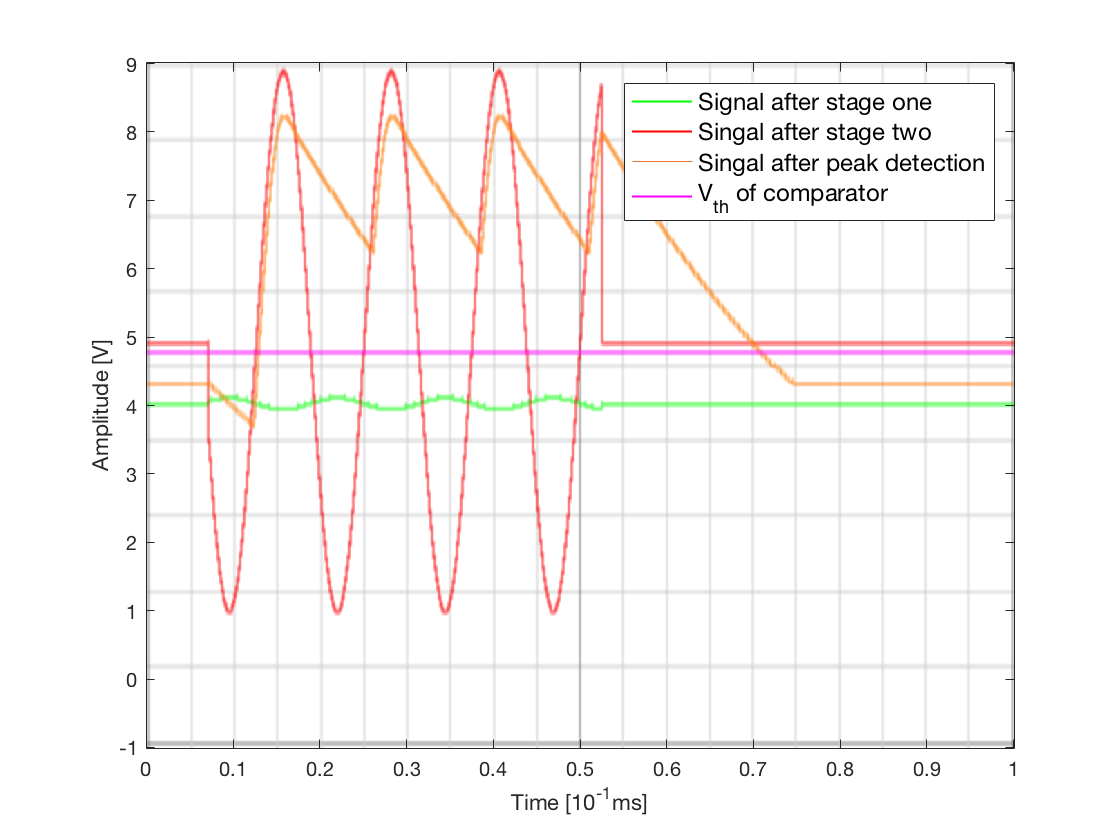
\includegraphics[width=1.0\textwidth]{Figures/receiver_simulations.PNG}
%   \caption{Operation amplifier signals}
%   \label{fig:sim_receive}
% \end{subfigure}%
% \begin{subfigure}{.5\textwidth}
%   \centering
%   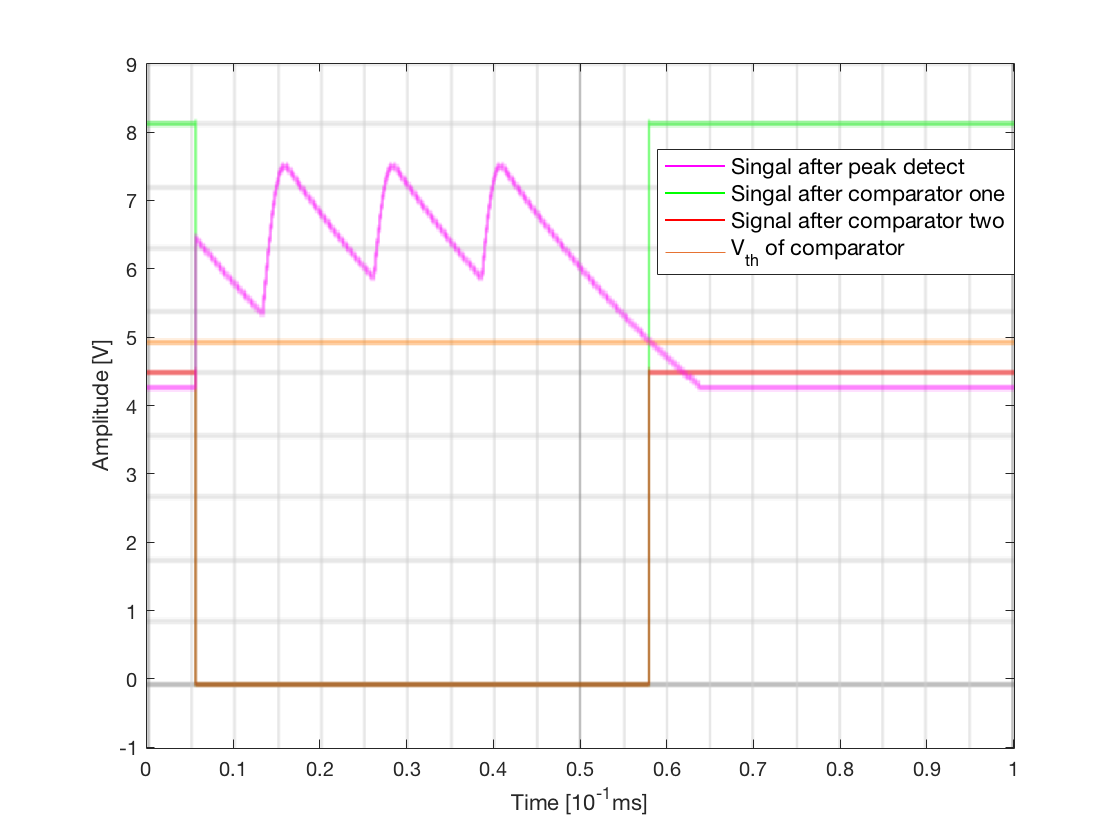
\includegraphics[width=1.0\textwidth]{Figures/receiver_simulations2.PNG}
%   \caption{Comparator signal}
%   \label{fig:sim_receive2}
% \end{subfigure}
% \caption{Simulation of receiver circuit}
% \label{fig:simulationreceiver}
% \end{figure}


Figure \ref{fig:sim_receive2} shows the signals of both comparator stages, together with the peak detection signal and the $V_{th}$ of the first comparator. No ultrasonic signal is detected between 0 and $0.05*10^{-1}ms^{-1}$, and a signal detected between $0.05*10^{-1}ms^{-1}$ and $0.5*10^{-1}ms^{-1}$ and after $0.5*10^{-1}ms^{-1}$ no ultrasonic signal is detected any more.
The comparators switch when the peak detection signal becomes higher than $V_{th}$ and the other way around. The second comparator has a $V_{th}$ of $2.5V$, so switches together with the signal of the first comparator stage. This switching is between the desired 0 and $5V$ for the micro controller.


\section{Conclusion}
From the simulations done in this chapter we can conclude that the antenna we are going to use for the prototype will have a \SI{50}{\degree} cone, since the reflections of this cone have the best horizontal reflecting characteristics. And together with that have the best transmitting and receiving characteristics.  The transmitting circuit not discussed in this part of the thesis, this because the transmitter IC \cite{MIC4428} isn't available in simulation software, so testing in real life is the way we are going to test the transmitting part. The receiver circuit works as we wanted in the simulations so we are going to make this circuit on a prototype solder board and test it in real life.

\chapter{Proof of concept}

This Chapter describes the design, manufacturing and testing of the proof of concept hardware.
Focus is put on verifying, where possible, the simulation results from Chapter \ref{chap:concept}.
During the test phase there might be multiple iterations to solve problems found during the tests.
These modification will be described and tested.
At the end of this chapter there should be enough confidence in the working of the system to start with a prototype design.

\section{Antenna}
\label{sec:antenna_proof}

The antenna is elevated above the ultrasonic transducer. It is important to centre the antenna lens and the transducer to make sure their axis align. For this purpose the transducer is centred on a circular mounting plate. The antenna is placed above the transducer by connecting it to two risers which are placed at fixed points in the mounting plate. The result is the antenna concept shown in Figure~\ref{fig:proto_ant}. The two risers could give the antenna a blind spot, later on we test if the risers have influence on the transmitting and receiving characteristics.
  Note that in this design the mechanical connection to the Zebro is not yet implemented. The final design with mechanical interface will be presented in the chapter describing the prototype, section \ref{sec:antennamech}.

\begin{figure}[H]
\centering
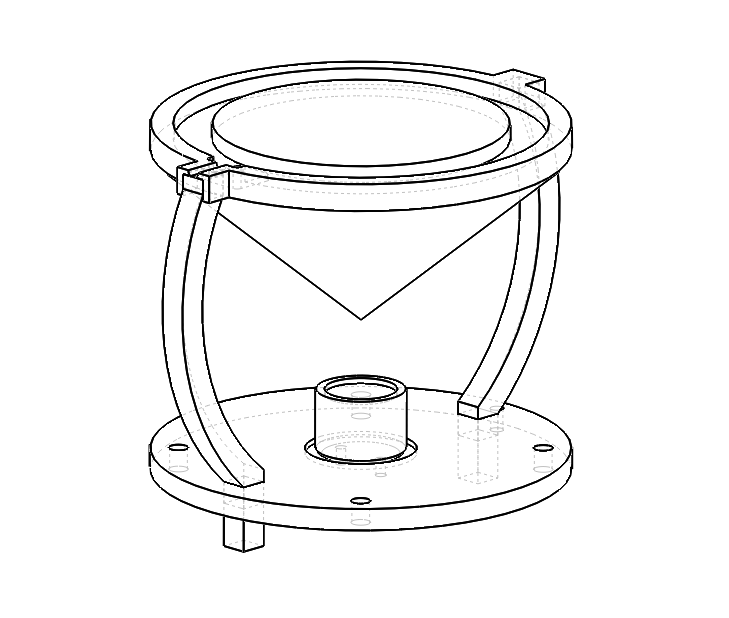
\includegraphics[width=0.6\textwidth]{Figures/proto_ant.PNG}
\caption{Proof of concept version of the ultrasonic antenna}\label{fig:proto_ant}
\end{figure}

Using that the beam pattern of the transducer is \SI{50}{\degree} we can find the distance between transducer and antenna for which the entire beam is incident on the antenna lens. Using the Zebro team 3D printer we made 2 copies of the antenna design, see Figure~\ref{fig:3D_ant}, to use for the proof of concept tests.

\begin{figure}[H]
\centering
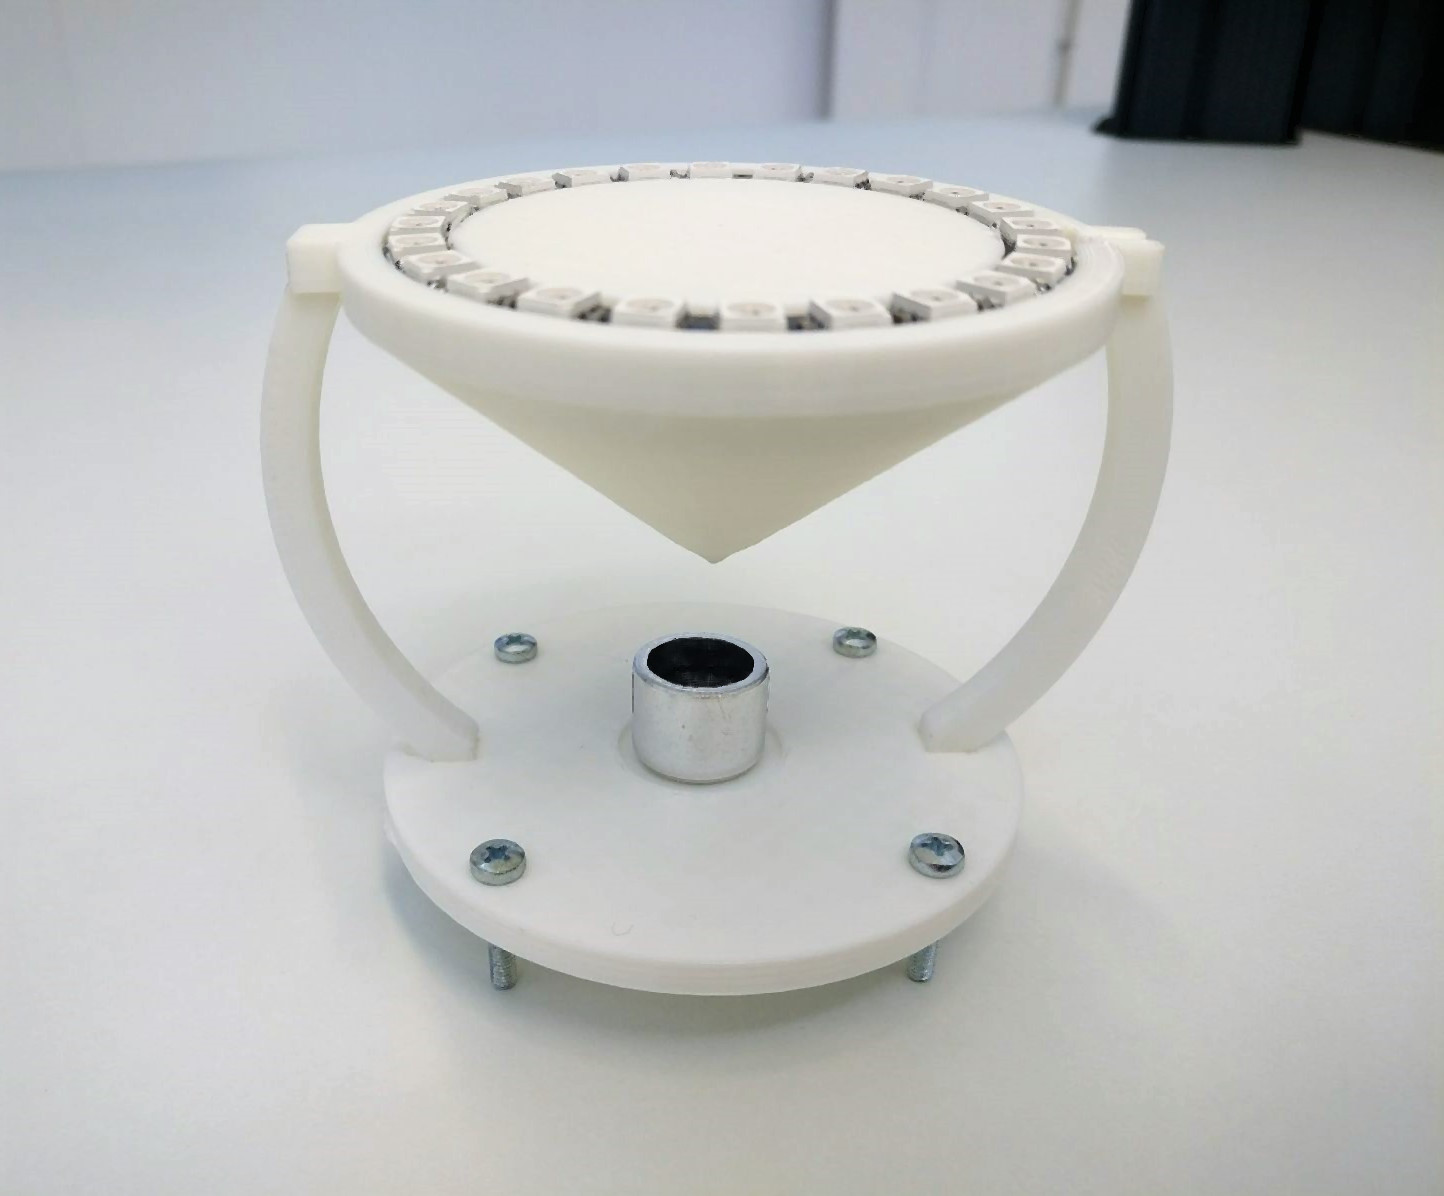
\includegraphics[width=0.6\textwidth]{Figures/3D_ant.jpeg}
\caption{3D printed proof of concept version of the antenna}\label{fig:3D_ant}
\end{figure}

The transmitter and receiver circuits can be connected to the bottom side of the mounting plate. The LED ring on top of the antenna is for human robot interaction purposes and can be used for system debugging and testing.


\section{Protoboard}

The circuit in Figure~\ref{fig:receivecircuit} is made on a protoboard as can be seen in Figure \ref{fig:protoboard}. The components used on the protoboard are components that were available in the Tellegenhall. For the operation amplifiers we used the LM741 \cite{LM741}, for the comparators we used a LM339 and a LM311. The rest of the components are normal resistors and capacitors. For the signals and power sources are cables soldered to the circuit. From left to right on the lower line in the circuit board, are the first and second stage amplifiers visible. Next to the amplifiers is the first stage comparator visible and on top the second stage comparator. On the board is also a potentiometer visible, because of this we can tune the amplification of the operational amplifier.


\begin{figure}[H]
\centering
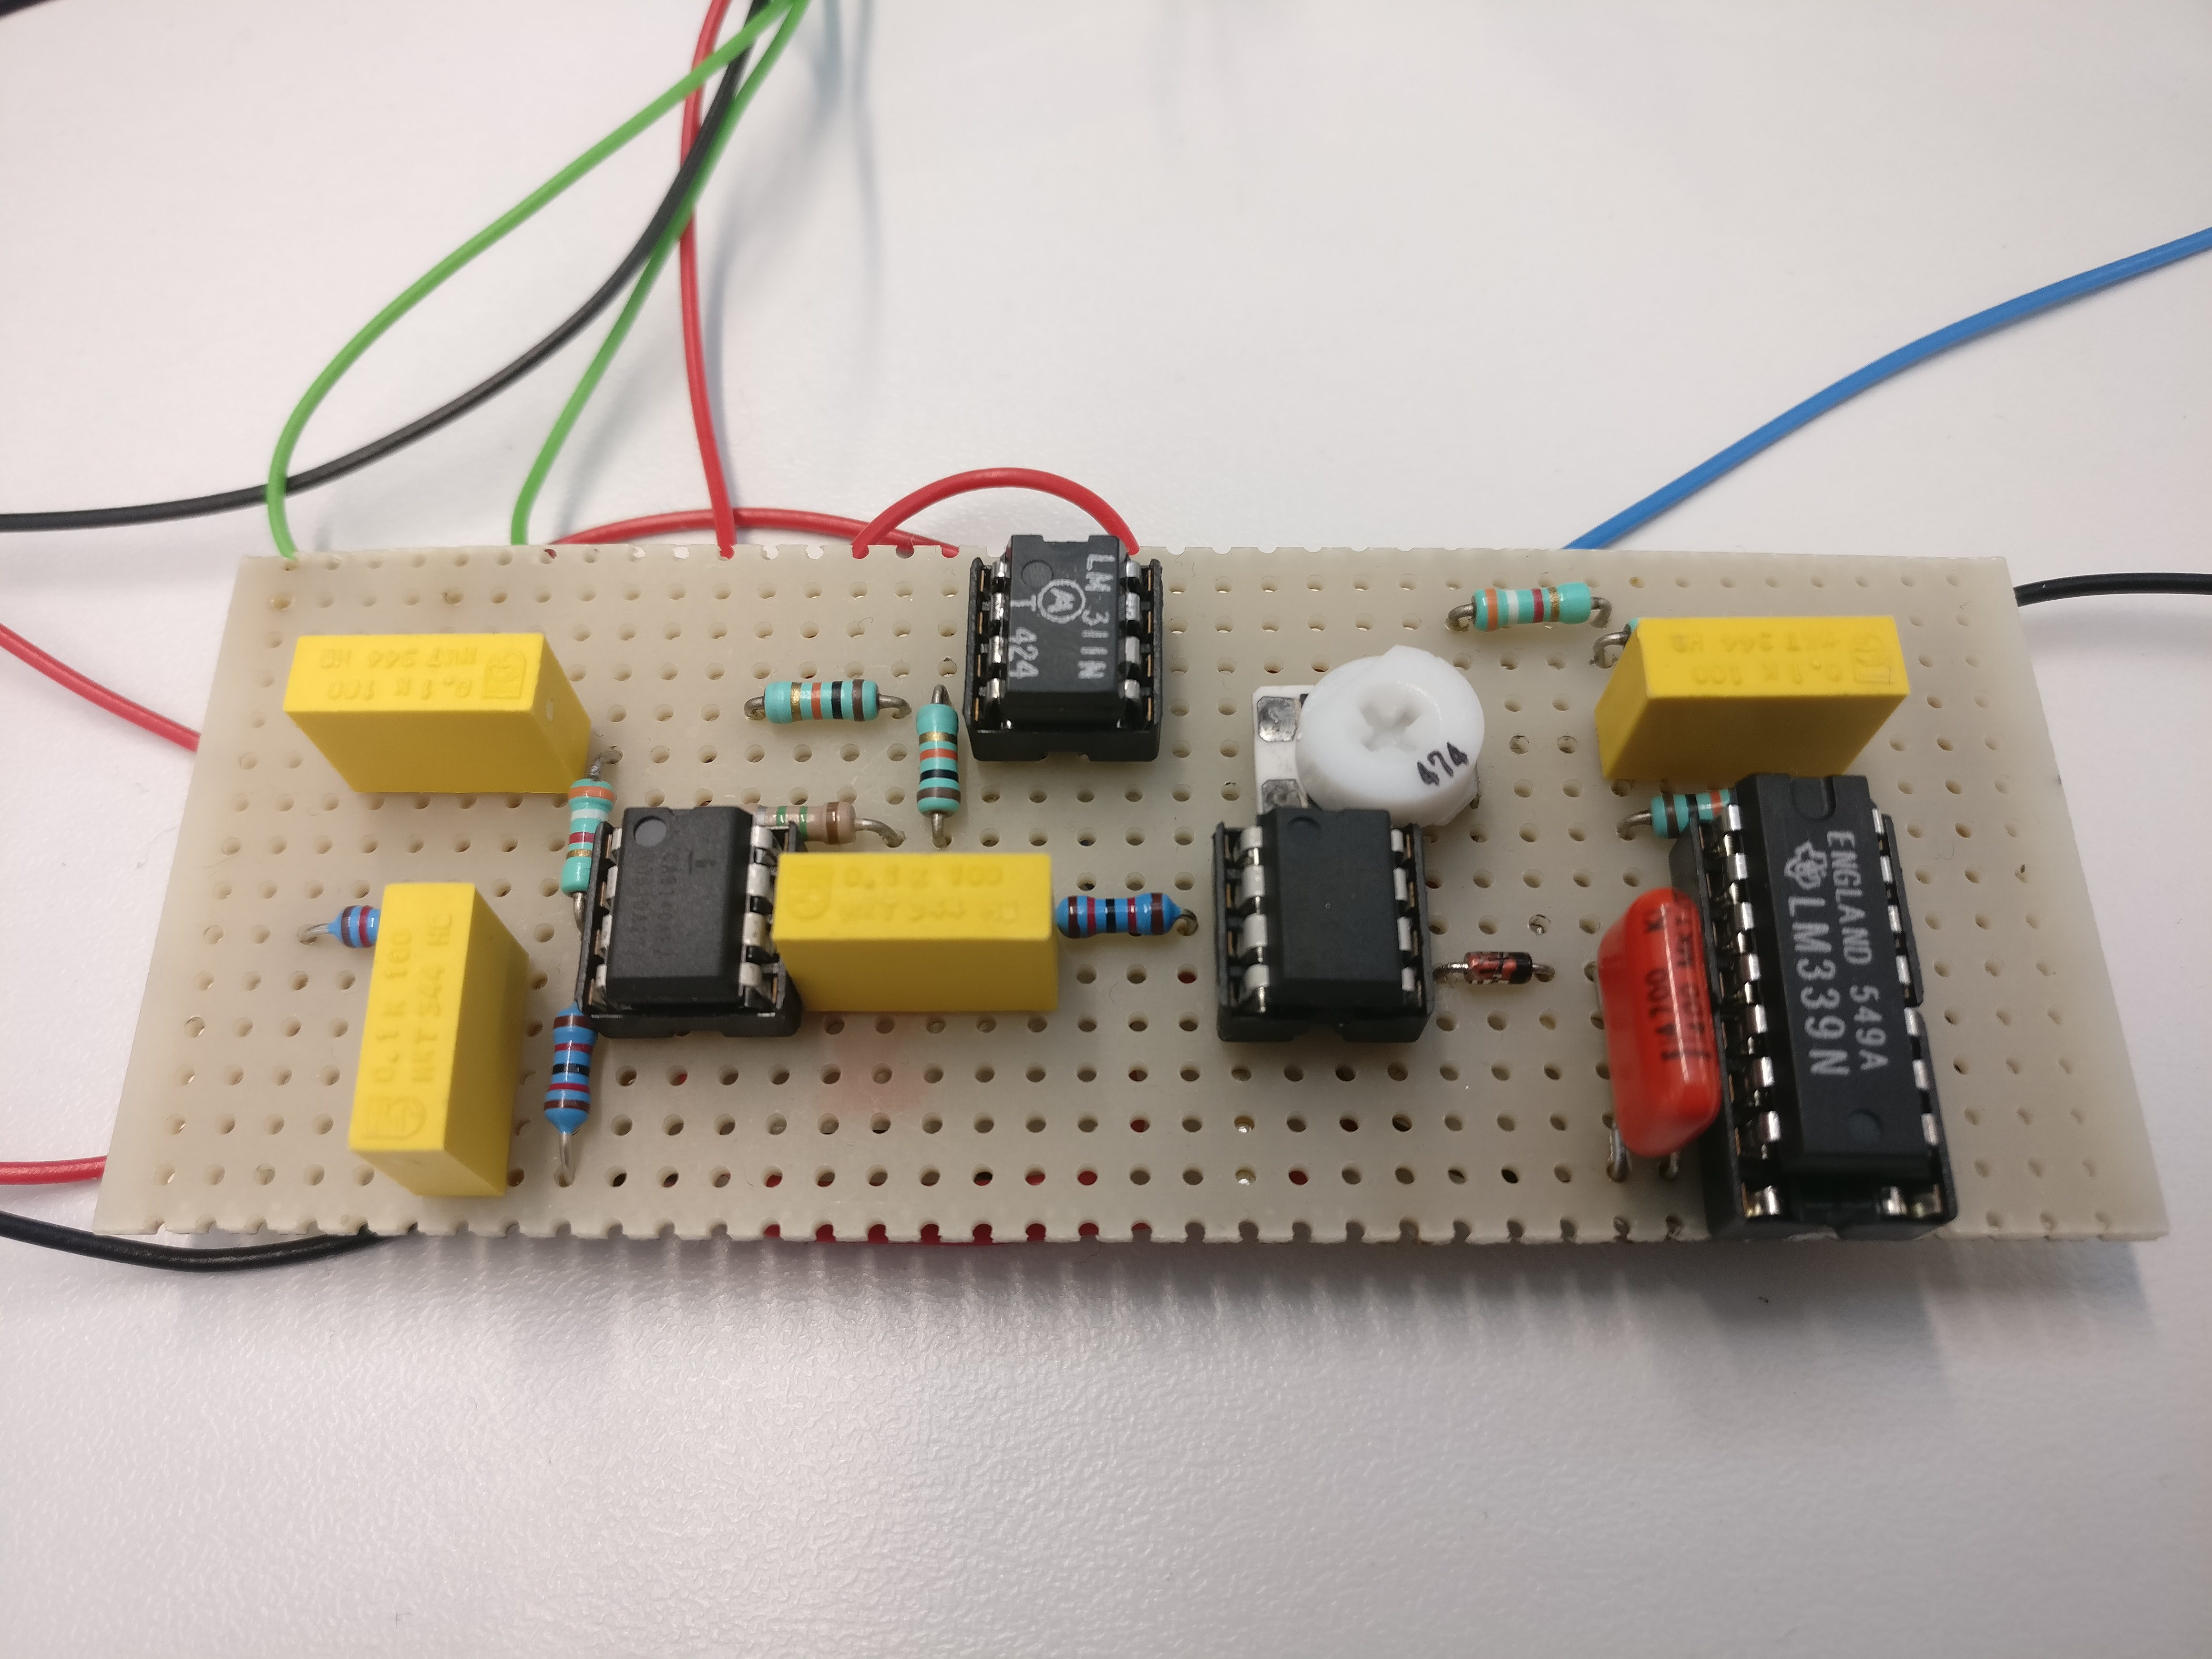
\includegraphics[width=0.6\textwidth]{proof_proto.jpg}
\caption{Proto board for the proof of concept receiver and detector circuit}\label{fig:proto}
\label{fig:protoboard}
\end{figure}

The protoboard of the transmitter circuit is simple, because it is a single MIC4428 \cite{MIC4428}
 IC, only the ultrasonic transceiver the power and signal wires are connected to it.

\section{Test plan}
The first test is to measure the internal signals of the circuit.
Using an oscilloscope we measure the signal at several points: the input, after each amplification stage, in the peak detection circuit and at the output to verify the correct working of the circuit.
In this test stage we check for production errors such as short circuits and check the component selection.

For the proof of concept tests the communication subsystem is not yet implemented.
This means that we cannot test the full concept as described in chapter~\ref{chap:concept} since we lack the required RF message.
We can however test the generation and accuracy of the $US_{detect}$ signal as seen in Figure~\ref{fig:ultra3}.
The $US_{detect}$ signal must have a clear distinction between a high (no pulse received) and low state (pulse received).
This change from high to low happens when the transducer receives a ultrasonic signal.

To test the circuit we connect it to a transducer placed in the reflecting antenna (Figure~\ref{fig:3D_ant}).
The output of the receiver circuit is the $US_{detect}$ signal.
To simulate the transceiver we power the MIC4428 \cite{MIC4428}
H-bridge driver IC with a power supply and use the signal generator to simulate the \SI{40}{\kilo\hertz} PWM wave output of the micro controller (see Figure~\ref{fig:ultra3}).
The output of the bridge driver IC is connected to a second ultrasonic transducer.

To see the effect the surroundings have on the distance measurements and thus on the $US_{detect}$ signal we perform the test in different set-ups:

\begin{itemize}
\item
Direct orientation with no reflecting surfaces or obstacles near the transmitter and receiver.
\item
The transmitter is placed close to a reflecting surfaces creating multiple paths from the transmitter to the receiver.
The reflecting surfaces are placed such that the extra paths are close in length to the original path.
\item
The transmitter and receiver are placed 7 meters apart with multiple obstacles, such as chairs and members of our bap group, in the direct path.
\end{itemize}

Using an oscilloscope we measure the $US_{detect}$ signal at the output of the receiver circuit.
By setting to oscilloscope to trigger at a falling edge we can visualise the change in the $US_{detect}$ signal.
The resulting measurements are given, and discussed, in the next section.

\section{Results}

When the receiver circuit receives a signal we see the expected \SI{4.5}{\volt} with the incoming signal modulated over it at the receiver input.
The incoming signal is, depending on the distance between transmitter and receiver, in the order of a few millivolt.
The signal is amplified by the first and second stage resulting in a $9V_{p-p}$ sinusoidal wave with an offset of \SI{4.5}{\volt} at the output of the second stage.

When the receiver circuit is not receiving we noticed something strange, instead of the \SI{4.5}{\volt} DC we would expect we see an sinusoidal wave at the output of the second stage.
The origin of this signal is the first amplifier.
While the first amplifier stage has \SI{4.5}{\volt} DC on both input pins it's output is a sinusoidal wave.
We assume that this signal is a noise signal resulting from a bad choice of operational amplifiers.
Since the circuit now generates a sinusoidal wave in both the receiving (intended) and not receiving (noise) state it's impossible to detect an ultrasonic pulse. When receiving an ultrasonic pulse we noticed that the amplification was not the amplification we expected, the amplification was lower.
Modifications need to be made to remove or filter this noise signal and get a higher op-amp amplification.


\begin{figure}[H]
\centering
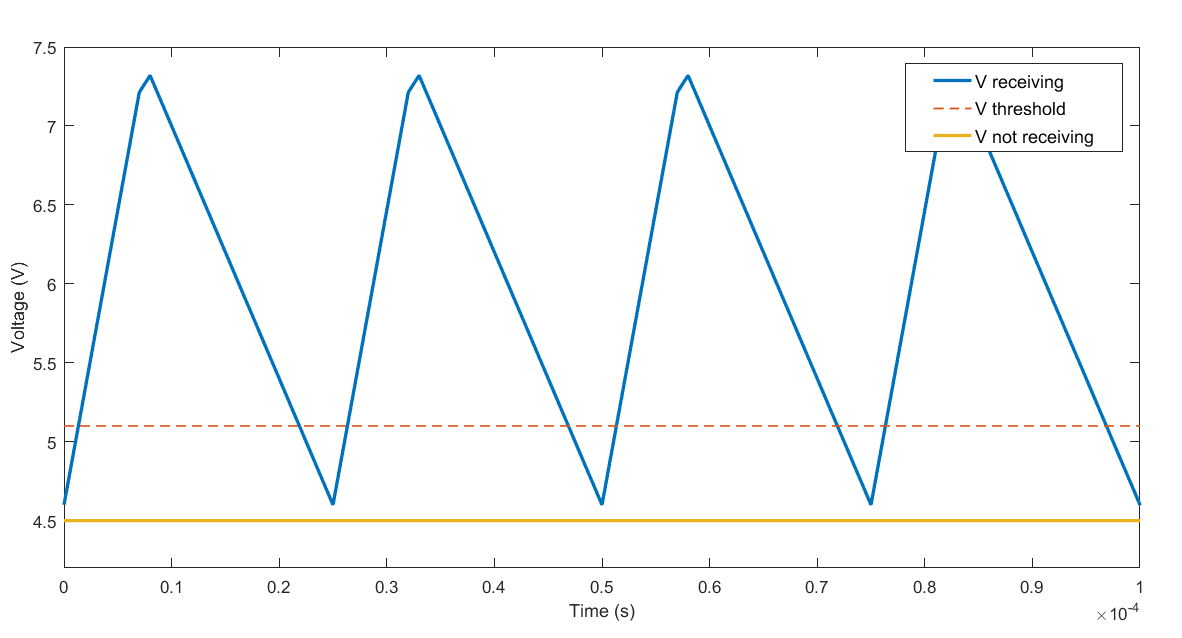
\includegraphics[width=0.9\textwidth]{Figures/waves_peak_detect_test.png}
\caption{Effect of a high peak to peak voltage output of the peak detect circuit}
\label{fig:waves_peak_test}
\end{figure}

When the circuit is receiving, the waveform at the output of the peak detection circuit has a higher peak to peak voltage and a lower mean than expected.
Due this high peak to peak voltage the signal at the input of the comparator goes below the threshold voltage each capacitor charge-discharge cycle (see Figure~\ref{fig:waves_peak_test}).
Thus the signal at the output, $US_{detect}$, is constantly switching between the high (not receiving) and low (receiving) state.
This can be solved by making some modification to the component values in the peak detection circuit.
The modifications made to the amplifiers and the peak detection circuit will be discussed in the next section.


\subsection{Modifications}
\label{chap:mod}
As discussed in the previous section the first prototype did not have the desired results. The first operational amplifiers produces a small oscillating signal which is amplified by the second stage op-amp. This oscillating signal could come from the resistor capacitor combination before the first op-amp or by the low bandwidth, gain bandwidth product of the LM741's. The voltage gain falls rapidly with increasing the signal frequency. At 40 kHz the gain of the LM741 is only 25 times. The LM741's are made for sound amplification that is having a maximum at 22 kHz The replacement operational amplifier, the LF353 \cite{LF353}, has a higher bandwidth which results in a higher possible voltage gain. With this modification the noise oscillation, as discussed in the previous section, is not noticeable any more. So this modification fixed the low gain and distortion signal for the peak detection circuit.

The problem with the peak detection circuit came from the fact that the capacitor discharges to fast. This is solved to change the discharge resistor to a higher value\footnote{The final values of the resistor is given in the circuit of appendix \ref{Appendixcircuits}.}, this way the capacitor discharges slower and the output signal of the peak detection circuit doesn't fall underneath the $V_{th}$ anymore.


\subsection{Results after modifications}

Figure~\ref{fig:proof_test_1} gives the results for the set-up without obstacles or reflections.
In this case there is a clear difference between the high and low state which can be detected by the micro controller.

\begin{figure}[H]
\centering
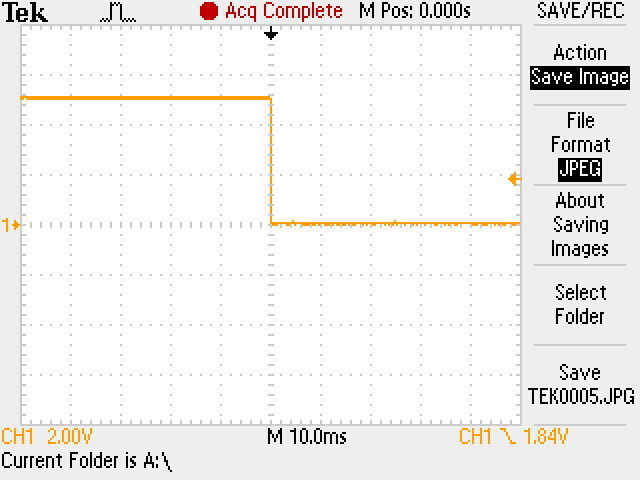
\includegraphics[width=0.6\textwidth]{test_proof_1.JPG}
\caption{Proof of concept test of US detect signal in direct orientation}\label{fig:proof_test_1}
\end{figure}

If the transmitter and receiver are placed in a less favourable set-ups with reflections and obstacles.
The low state of the $US_{detect}$ signal is not always stable. %cancellation
Due to the reflections and obstacles the transducer does not receive the entire pulse, either because parts are blocked or have destructive interferences from the multiple paths caused by the reflections.
This instability might cause measurements to fail or become inaccurate since the micro controller might see the signal as high instead of the low corresponding to receiving.
We estimate the effect of this instability to be negligible since:

\begin{itemize}
\item
Only the first falling edge is important, this is the most direct path the ultrasonic signal travels. The distortions mostly result out of reflections and signal cancellations, but these signals are never the direct path of the signal. This is why these instabilities can be neglected.
\item
Since we want to have an accuracy of 10cm over the distance of 1 meter. We need to poll at a certain frequency. The speed of sound is \SI{343}{\meter}$s^{-1}$, the time it takes for sound to travel 10 cm is 0.29ms. This is why we will use a clock of \SI{40}{\kilo\hertz} for the polling, this frequency does have period of 0.025ms and thus can reach an accuracy of $343 * 0.025 = 8.6 mm$ in ideal conditions.
The received noise is in the order of mili seconds. This means that we might do a miscount due to the noise but the error will be in the order of \SI{25}{\micro\second}.
To miss an entire measurement the noise would have to perfectly align with the counter cycle such that the signal is high every time the counter checks the $US_{detect}$ signal.
We assume the chances for this to happen are low but at this point in time we cannot yet measure the influence of the noise since the communication subsystem and micro controller are not yet integrated.
As soon as we have a working system prototype, with all subsystems integrated, we can test how often a measurement fails due to the noise.
\item
Since the speed of the Zebro is low, \SI{5}{\meter\per\second}, and the frequency of measurements is high a neighbouring Zebro will not have moved out of communication range when one measurement is failed.
It is not necessary to know the accurate location of each neighbour as long as the Zebro know that he is within communication range of others.
\item
The processing method, a particle filter, has capabilities to detect missed measurements and to act accordingly. \cite{processing}
\end{itemize}

\begin{figure}[H]
\centering
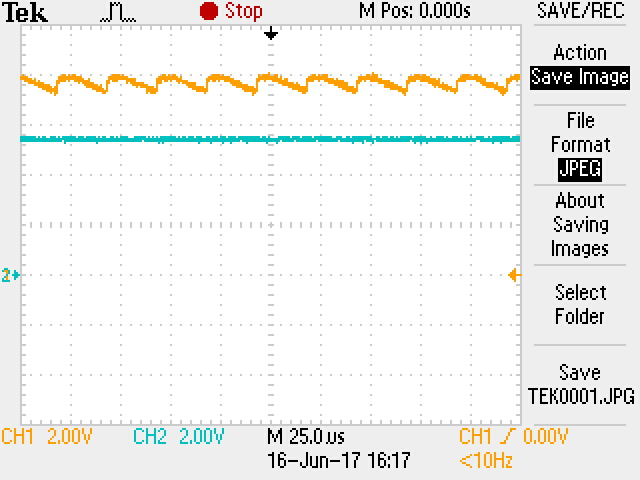
\includegraphics[width=0.6\textwidth]{Vth_Vpeak.JPG}
\caption{Peak detect signal together with the $V_{th}$ of the first comparator when receiving}\label{fig:peakvth}
\end{figure}

The peak detection circuit was also being modified and gives a much better result now. As can be seen in Figure \ref{fig:peakvth}, the peak detect signal (Yellow) stays high when receiving a pulse the capacitor discharges slowly enough to keep the signal above the $V_{th}$ (Blue) of the first comparator. The zero reference is turned 1 division down to get a better plot. So the $V_{th}$ is around 5.2V.

As discussed in section \ref{sec:antenna_proof} the risers of the antenna could give the antenna a blind spot, however with testing we didn't recognise any influence on the transmitter and receiver side due to these risers.

\section{Conclusion}
From the test we have done we can conclude that the transmitter and receiver concept prototypes work after the needed modifications. The task now is to combine the both circuits to a working prototype.
The antenna works properly as well as we can see from the results. With simple test the range of the transmitter and receiver can reach easily 5 meters.
The only remark that can be made is that the both comparators don't have hysteresis implemented yet. This is done because the $V_{th}$ of the first comparator is close to the voltage of the not receiving signal. This results in the situation that the hysteresis region becomes small. This is why in this stage of the project is chosen to leave the hysteresis in the comparators away.

\addtocontents{toc}{\protect\newpage}
\chapter{Prototype}
In this chapter the development of the prototype is described.
This prototype will be delivered to the Zebro team, so should conform to all the interface requirements given in chapter~\ref{chap:por}.
The first step is to integrate the transmitter and receiver circuits and design the necessary power circuitry.
The next step is to link our distance measurement system to the communication system \cite{communication} and the processing system \cite{processing}.
Before we order the prototype PCB of the full system we test the systems on a naked prototype PCB produced with the PCB milling machine of the Zebro team.
This naked prototype PCB allows us to test if the systems will work on a PCB with surface-mounted devices (SMD) components.

Using the naked prototype PCBs we will test the prototype module in phases.
The test phases are described at the end of this chapter in section \ref{sec:testplan}.
The test results will be given in Chapter~\ref{chap:results}.

\section{Subsystem integration}

\subsection*{Switching between transmitting and receiving}

To integrate the receiver and transmitter circuit a switching circuit is required as shown in the overview in figure~\ref{fig:ultra3}.
The switching circuit switches between transmitting and receiver mode.
When in transmitting mode the receiving circuit should be decoupled from the transducer to protect the receiver circuit from the $30V_{p-p}$ generated by the transmitter.

An option to switch the circuits on and off would be to switch their power supplies.
The problem with switching off the receiver by switching it's power supply off is that the input of the first op-amp is still $30V_{p-p}$.
This might create unpredictable and undesirable op-amp outputs or even damage the op-amps.
Simply switching off a power supply is thus not an option.

A transistor is another commonly used component to switch. But, the difficult part is that the polarity is not fixed for the transistor. This makes it not the best option for switching between the transmitter and receiver circuit.

A relay could be used to mechanically switch the system from transmit mode to receive mode.
The advantage is that, by using a relay, the circuits are decoupled thus protecting the receiver circuit from the output of the transmitter circuit.
Problem is that relays are rather large and not available in a SMD package.

An analogue switch, also called a bilateral switch, is an alternative to the relay.
A bilateral switch basically is a relay without moving parts and available in a small SMD package.
As a comparison, the SMD bilateral switch package contains 3 switches but is smaller than a single relay.
To switch between the two modes we need 2 switches, one for each pin of the transducer.
The only reason to use a relay instead of the bilateral switch would be to switch high currents.
Since the circuit is not switching high currents the bilateral switch is the best option for our switching circuit.
The resulting circuit with implemented bilateral switches is given in section~\ref{sec:proto_circuit}.

\subsection*{Power supply}

The circuit requires 3 voltage levels:
\begin{itemize}
\item
\SI{5}{\volt} to power the second comparator in the receiver circuit.
\item
\SI{9}{\volt} to power the op-amps and the first comparator in the receiver circuit and to create the \SI{4.5}{\volt} bias for the receiver circuit.
\item
\SI{15}{\volt} for the power supply of the H-bridge driver IC in the transmitter circuit and the bilateral switches.
\end{itemize}

The \SI{5}{\volt} is a voltage used in all three systems as most ICs, such as the micro controller required for processing and operating the module, require a \SI{5}{\volt} power supply.
This voltage is thus created for all systems using a basic voltage regulator circuit (LDIO).
The creation of this \SI{5}{\volt} line is describe in the paper of the communication system \cite{communication}.

The \SI{15}{\volt} and \SI{9}{\volt} level are only present in the distance sensing system.
We use two voltage regulators to create the stable voltage levels from the changing Zebro battery voltage. %ref to battery requirement.
These regulators are implemented in the circuit presented in section~\ref{sec:proto_circuit}.

\section{System integration}
\label{sec:sys_int}

\begin{figure}[H]
\centering
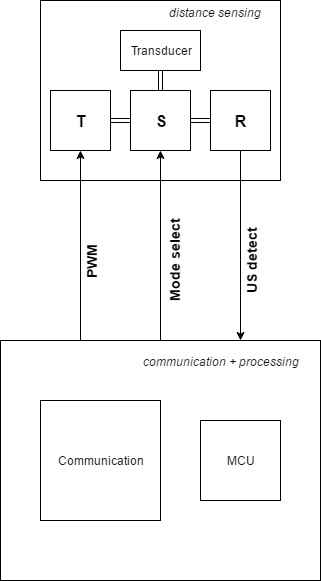
\includegraphics[width=0.5\textwidth]{Figures/integration.png}
\caption{Data link between the distance sensing system and the rest of the module}
\label{fig:int}
\end{figure}

Figure~\ref{fig:int} shows the data link between the distance sensing module described in this paper and the other systems in the module.
The figure shows:

\begin{itemize}
\item
\textbf{T} The transmitter circuit as described in section~\ref{chap:trans}.
\item
\textbf{R} The receiver circuit as described in section~\ref{chap:receiver}.
\item
\textbf{S} The switching circuit witch switches the transducer between the transmitter and receiver circuit.
\item
\textbf{PWM} \SI{40}{\kilo\hertz} \SI{50}{\percent} PWM wave generated by the microcontroller (MCU). This wave is amplified by the transmitter circuit to drive the ultrasonic transducer.
\item
\textbf{Mode select} Control signal from the MCU which selects the desired mode: transmit or receive. This is a \SI{5}{\volt} signal which switches the bilateral switches.
\item
\textbf{US detect} Data signal which tells the microcontroller if a ultrasonic pulse is received. This signal has two levels: \SI{5}{\volt} not receiving and \SI{0}{\volt} receiving.
\end{itemize}

These data connections, together with the power rail connections, connect the distance sensing module to the other systems in the module.
The MCU decides when an ultrasonic pulse has to be sent and actives the corresponding signals: the PWM signal to generate the signal needed to drive the transducer and the mode select signal to select the transmitter mode.
When the communication module receives an RF message from another Zebro telling it an ultrasonic pulse is incoming the MCU selects the receive mode and listens to the $US_{detect}$ signal.
How these data links are connected is explained in section~\ref{sec:proto_circuit}.

\section{Prototype circuit}
\label{sec:proto_circuit}

In appendix \ref{Appendixcircuits} is the total ranging circuit visible. This includes: the transmitter circuit, the switching circuit, the receiver circuit and the desired voltages together with some connectors. The modifications discussed before in section \ref{chap:mod} are all implemented in the circuits. When the circuits were ready, the layout of the printed circuit board was made to get a working naked prototype out of the PCB milling machine. The PWM signal as mentioned in the section before is the PWM40kHz signal in the circuit, the mode select signal is the ON/OFF signal in the circuit and the US detect signal is the output signal of the circuit.
Since all the components are known now, a bill of materials is made and visible in appendix \ref{AppendixBOM}
The total costs of all the components for a ranging circuit sums up to \euro11,57 per circuit.


\section{Module housing and antenna}
\label{sec:antennamech}

\begin{figure}[H]
\centering
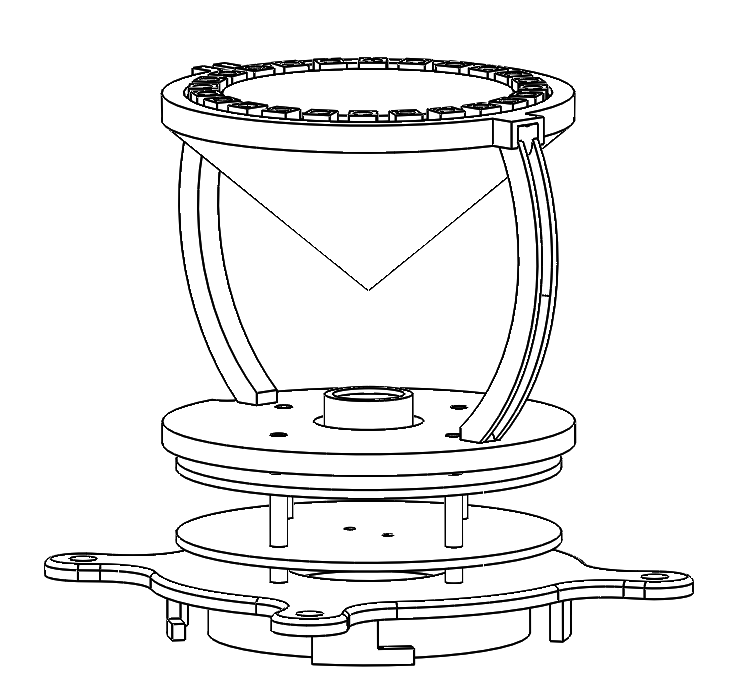
\includegraphics[width=0.8\textwidth]{Figures/prototype_ant.PNG}
\caption{3D model of the module prototype}
\label{fig:proto_module}
\end{figure}

To mechanically fasten the module to the Zebro a twist lock connection is required as described in the deci Zebro interface document~\cite{DeciSpecs}.
The system PCB stack is connected to the twist lock with four M3 risers.
The ultrasonic transducer is placed on the top PCB and slides in the antenna base plate.
The antenna base plate is placed on top of the PCB stack by connecting it to the M3 risers.
An 3D overview of the final module prototype is given in figure~\ref{fig:proto_module}.

The current prototype is kept modular.
The size, height and number of PCBs in the stack can change freely as long as they have the 4 M3 holes required to connect to the risers.
This makes sure last minute changes in the PCB design do not influence the design of the other prototype parts such as the twist lock connector.

\section{Naked prototype PCB}

 Visible in figure \ref{fig:naked_pcb}, is the print layout of the naked prototype PCB. It is taken into account that it is just a prototype. So to make the PCB as small as possible is not the biggest concern. The main concern is that it is a PCB that is easily to solder by hand, and if there are small failures in the board, it could be easy fixed. Also is taken into account that the components are placed in is logically. So the power circuits are at the top left side of the PCB, the transmitter circuit is at the left bottom side, with in the middle of the PCB the bilateral switch and on the right side the receiver circuit.

\begin{figure}[H]
\centering
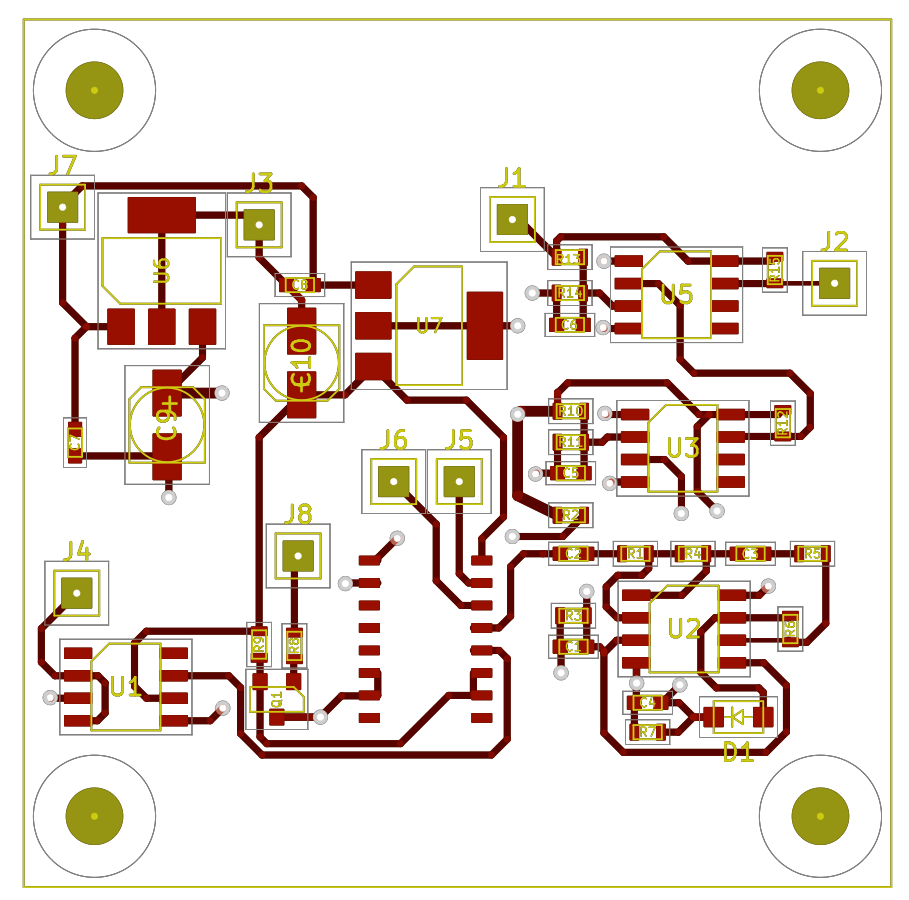
\includegraphics[width=0.6\textwidth]{Figures/Total_circuit.png}
\caption{Top layer of the naked proto PCB}
\label{fig:naked_pcb}
\end{figure}


\section{Problems during integration with communication system}
\label{sec:delay}
When testing the communication system the delay between giving the command to transmit a message an actually transmitting the message was found to be higher than expected.
During the concept design it was assumed that the RF message would be transmitted, and arrived at the other Zebro, instantaneous.
Test of the communication system showed that there is a delay of roughly \SI{6}{\milli\second} before the message was actually transmitted after the command was given.
This delay is likely due to the processing actions undertaken by the Digimesh modules to assure high mesh network communication performance.

The first problem this gives is a error of \SI{6}{\milli\second} in the measurement of $\Delta t$ (see figure~\ref{fig:ultra1}) since the ultrasonic pulse is now transmitted \SI{6}{\milli\second} before the RF message.
This gives an distance measurement result that is roughly \SI{2}{\meter} lower than the actual distance between the Zebros.

The second problem is that when the distance between the Zebros is low the ultrasonic pulse will now reach the other Zebro before the RF message does.
This means that the Zebro has not yet started the TDOA measurement since the RF message marks the start of the TDOA measurement.
The delay is \SI{6}{\milli\second} in which the ultrasonic pulse travels a distance of roughly \SI{2}{\meter}.
Thus when the distance between Zebros is smaller than \SI{2}{\meter} the ultrasonic pulse will arrive before the RF measurement thus resulting in a failed measurement.

Luckily the delay is roughly constant, it has a deviation of plus minus \SI{1}{\milli\second}, which makes it possible to work around this delay.
It is possible to:

\begin{itemize}
\item
Take the delay into account when calculating the distance form the measured $\Delta t$ by adding the delay to the measured $\Delta t$
This option provides no solution for the second problem: an ultrasonic pulse arriving before the RF message.
This means, when using this option, measurements cannot be done when the distance between Zebros is smaller than \SI{2}{\meter}.
\item
Adding the same delay to the transmission of the ultrasonic pulse such that the RF message and ultrasonic pulse are again transmitted simultaneously.
\item
Allowing both the RF message and the ultrasonic pulse to function as the $t_{0}$ timestamp for the TDOA depending on which arrives first.
This means that when the ultrasonic pulse arrives first we will measure the time difference between the arrival of the ultrasonic pulse $t_{0}$ and the arrival of the RF pulse.
Using the known value of the delay we can than calculate the distance between Zebros even if the ultrasonic pulse arrives before the RF message.
\end{itemize}

An attempt is made to implement the third option.
This option works for all distances, unlike the first option, and does not require the delay on the microcontroller the second option needs.
Implementing the delay on the microcontroller means that the microcontroller cannot undertake an other action during the \SI{6}{\milli\second} delay.
This would slow down the microcontroller and thus the system.

The implementation of this option is not discussed in this thesis since it is undertaken in the last 2 weeks of the bachelor end project after the deadline of the thesis.
We discuss the problem here since it will be included in the recommendations sections and it will influence the prototype testing phase as discussed in the next section.

\section{Test plan}
\label{sec:testplan}
Since the discussed option is not yet implemented for the first prototype tests, complete distance measurements cannot be performed.
Instead measurements are done by measuring the $US_{detect}$ signal and the communication signal using an oscilloscope.

Before we can test the distance measurements we first need to measure the delay in the communication channel and the deviation of this delay.
To measure the delay we plot the TX signal of the transmitting module and the RX signal of the receiving module on the oscilloscope.
From these 2 signals the delay between transmitting and receiving can be determined.

Using 2 modules equipped with the naked proto PCBs we measure the performance for 3 different distances.
First the modules are placed with a distance of \SI{1}{\meter} between them.
For the second test this distance is increased to \SI{3}{\meter} and to \SI{5}{\meter} for the final test.
By plotting the RX signal and the $US_{detect}$ signal of a single module on the oscilloscope the TDOA of the two signals can be determined.

Using the delay measured in the first test and the TDOA of the second test a distance can be calculated.
Focus is put on the deviation of the result when the measurement is performed multiple times.
It's less important if the result corresponds to the actual distance since, as long as the measurement deviation is small, the system can be calibrated to give the correct distance.
Using the deviation measured on the communication delay it is possible to determine if a deviation in the distance result is due to the communication system or the distance sensing system.

For the test the microcontroller is simulated by an Arduino to generate the control and data signal necessary for the test.
For the distance sensing system (transmitter + receiver) the naked proto PCBs are used.
The communication system is implemented with an protoboard and the Digimesh modules as discussed in the thesis regarding the communication system \cite{communication}.
The necessary power is supplied by multiple power supplies.

\chapter{Results}
\label{chap:results}

\section{Test plan}
\label{sec:testplan}
Since the countermeasure against the delay in the communication channel is not yet implemented for the first prototype tests, complete distance measurements cannot be performed.
Instead measurements are done by measuring the $US_{detect}$ signal and the communication signal using an oscilloscope.

Before we can test the distance measurements we first need to measure the delay in the communication channel (RF) and the deviation of this delay.
To measure the delay we plot the TX signal of the transmitting module and the RX signal of the receiving module on the oscilloscope.
The TX signal shows when a module starts transmitting packages over the RF channel and the RX signal shows when the other module starts receiving the packages.
We do this measurement over an arbitrary distance.
From these 2 signals the delay between transmitting and receiving can be determined.

Using 2 modules equipped with the naked proto PCBs we measure the performance for 3 different distances.
First the modules are placed with a distance of \SI{1}{\meter} between them.
For the second test this distance is increased to \SI{3}{\meter} and to \SI{5}{\meter} for the final test.
By plotting the RX signal and the $US_{detect}$ signal of a single module on the oscilloscope the TDOA of the two signals can be determined.

Using the delay measured in the first test and the TDOA of the second test a distance can be calculated.
Focus is put on the deviation of the result when the measurement is performed multiple times.
It's less important if the result corresponds to the actual distance since, as long as the measurement deviation is small, the system can be calibrated to give the correct distance.
Using the deviation measured on the communication delay it is possible to determine if a deviation in the distance result is due to the communication system or the distance sensing system.

For the test the microcontroller is simulated by an Arduino to generate the control and data signal necessary for the test.
For the distance sensing system (transmitter + receiver) the naked proto PCBs are used.
The communication system is implemented with an protoboard and the Digimesh modules as discussed in the thesis regarding the communication system \cite{communication}.
The necessary power is supplied by multiple power supplies.

\section{Measurements}

\begin{figure}[H]
\centering
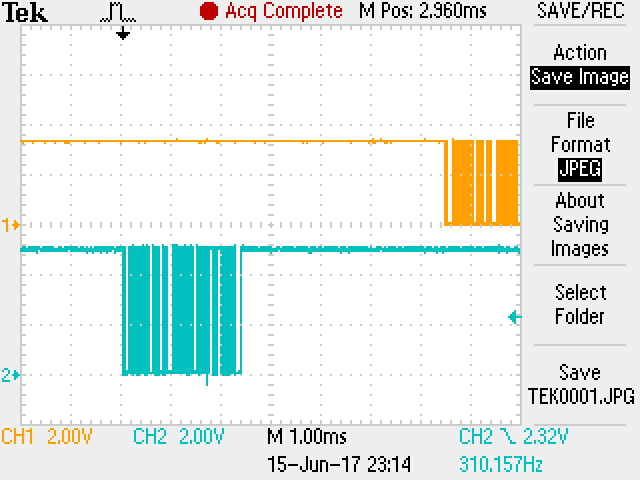
\includegraphics[width=0.8\textwidth]{Figures/delay_tx_rx.JPG}
\caption{Delay in TX an RX (RF communication channel)}
\label{fig:delay_tx_rx}
\end{figure}

Figure~\ref{fig:delay_tx_rx} shows the TX signal of the transmitting module (Blue) and the RX signal of the receiving module (Yellow).
The delay between transmitting a package and receiving the package at the other module is \SI{6.5}{\milli\second}.
Due this delay there is a difference of \SI{6.5}{\milli\second} between the measured TDOA and the actual $\Delta t$ (see figure~\ref{fig:ultra1}) as discussed in section~\ref{sec:delay}.
This means the distance error corresponding to the measured delay is:

$ v_{sound} * t_{delay} = \SI{340.29}{\meter\per\second} * \SI{6.5}{\milli\second} = \SI{2.2}{\meter} $

Since this delay is present in every measurement there will be an error of \SI{2.2}{\meter} in every measurement.
The distance corresponding to the delay, \SI{2.2}{\meter}, will be added the to result of the distance measuring test to show that the measurements are correct when the delay is taken into account.
At this point this has to be done manually but in the future a method to deal with this delay will be implemented as discussed in section~\ref{sec:delay}.

When we perform the measurement of the delay between TX and RX multiple times with different distances between the two modules we notice the following:

\begin{itemize}
\item
The delay is independent of the distance between transmitter and receiver.
\item
The delay varies with time.
It has an average of \SI{6.5}{\milli\second} and a deviation of \SI{0.5}{\milli\second}.
This means that for every measurement the actual delay in the communication channel will lie somewhere between \SI{6}{\milli\second} and \SI{7}{\milli\second}.
For each measurement the actual value for this delay will be different and thus introduces an inaccuracy.
\end{itemize}

This means that, by using the average delay to compensate for the effect of the delay, a maximum error of $\pm$ \SI{0.5}{\milli\second} is introduced to $\Delta t$.
This error corresponds to a distance error of:

$ v_{sound} * \pm t_{error} = \SI{340.29}{\meter\per\second} * \pm \SI{.5}{\milli\second} =\pm \SI{20}{\centi\meter} $


\begin{figure}[H]
\centering
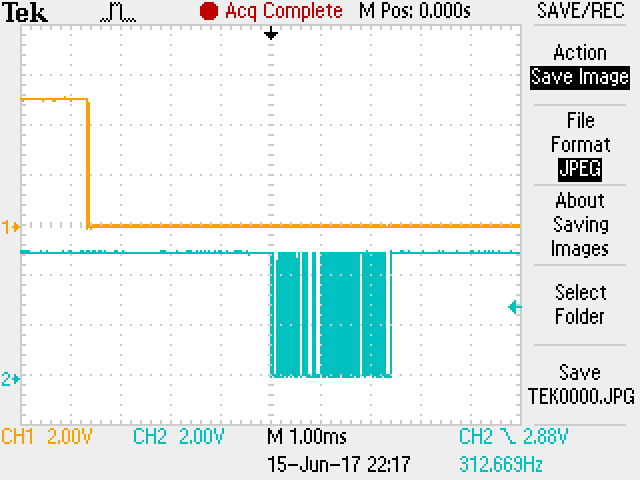
\includegraphics[width=0.8\textwidth]{Figures/test_1m.JPG}
\caption{Measurement with a distance of \SI{1}{\meter} between modules}
\label{fig:mes_1}
\end{figure}

Figure~\ref{fig:mes_1} shows the $US_{detect}$ signal (Yellow) and the RX signal (Blue) of a single module.
The falling edge in the $US_{detect}$ signal is the time at which a ultrasonic pulse is first detected.
Since the distance between the modules is smaller than the distance corresponding to the delay, the ultrasonic pulse arrives at the module before the start package of the RF message.
The TDOA between the ultrasonic pulse and the start of the RF message is \SI{3.6}{\milli\second}.
Since the RF message is transmitted \SI{6.5}{\milli\second} after the ultrasonic pulse $\Delta t$ can be calculated by, in this case, by subtracting the measured TDOA from the delay.
This gives a $\Delta t$ of:

$ \Delta t = t_{delay} - TDOA = \SI{6.5}{\milli\second} - \SI{3.6}{\milli\second} = \SI{2.9}{\milli\second} $

Which corresponds to a distance of:

$ v_{sound} * t_{delay} = \SI{340.29}{\meter\per\second} * \SI{2.9}{\milli\second} = \SI{1}{\meter} $

Although the resolution of the measurement is low since the TDOA is estimated with the oscilloscope (to one decimal) it shows that the distance measurements are correct when the delay is taken into account.
In the fully integrated prototype these TDOA measurements will be done with a microcontroller resulting in a higher resolution.
Unfortunately this hardware is not available at the point of writing so it's impossible to make conclusions on the accuracy of the measurement.

\begin{figure}[H]
\centering
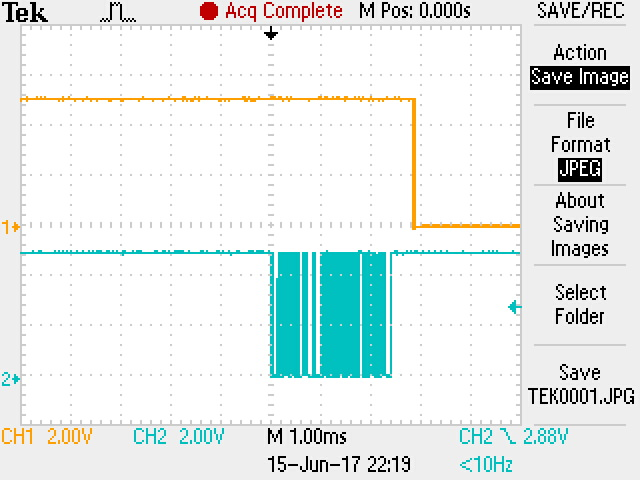
\includegraphics[width=0.8\textwidth]{Figures/test_3m.JPG}
\caption{Measurement with a distance of \SI{3}{\meter} between modules}
\label{fig:mes_3}
\end{figure}


Figure~\ref{fig:mes_3} shows the $US_{detect}$ signal (Yellow) and the RX signal (Blue) of a single module for the second measurement done for a distance of \SI{3}{\meter}.
In this case the distance is larger than the distance corresponding to the delay so the ultrasonic pulse arrives after the RF message.
The TDOA between the start of the RF message and the ultrasonic pulse is \SI{2.8}{\milli\second}.
Since the RF message is transmitted \SI{6.5}{\milli\second} after the ultrasonic pulse $\Delta t$ can be calculated by, in this case, adding the delay to the measured TDAO.
This gives a $\Delta t$ of:

$ \Delta t = TDOA + t_{delay}  = \SI{2.8}{\milli\second} + \SI{6.5}{\milli\second} = \SI{9.3}{\milli\second} $

Which corresponds to a distance of:

$ v_{sound} * t_{delay} = \SI{340.29}{\meter\per\second} * \SI{9.3}{\milli\second} = \SI{3.2}{\meter} (\Delta = \SI{20}{\centi\meter} $ compared to the actual distance of $\SI{3}{\meter})$

\begin{figure}[H]
\centering
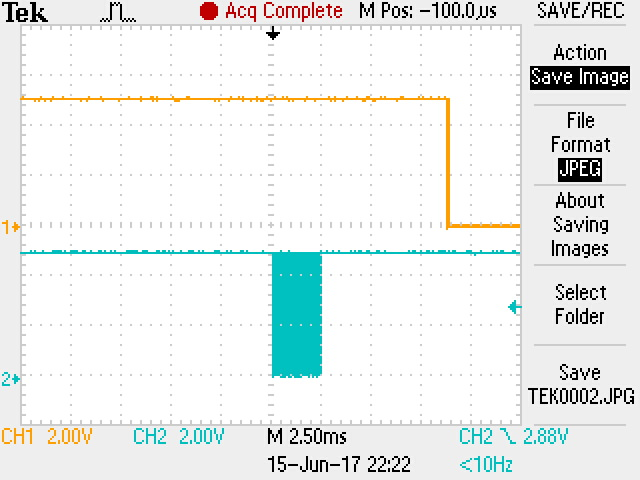
\includegraphics[width=0.8\textwidth]{Figures/test_5m.JPG}
\caption{Measurement with a distance of \SI{5}{\meter} between modules}
\label{fig:mes_5}
\end{figure}

Figure~\ref{fig:mes_5} shows the $US_{detect}$ signal (Yellow) and the RX signal (Blue) of a single module for the third measurement done for a distance of \SI{5}{\meter}.
Note that the scale is different than the first two measurements.
The TDOA between the start of the RF message and the ultrasonic pulse is \SI{8.8}{\milli\second}.
Since the RF message is transmitted \SI{6.5}{\milli\second} after the ultrasonic pulse $\Delta t$ can be calculated by, in this case, adding the delay to the measured TDAO.
This gives a $\Delta t$ of:

$ \Delta t = TDOA + t_{delay}  = \SI{8.8}{\milli\second} + \SI{6.5}{\milli\second} = \SI{15.3}{\milli\second} $

Which corresponds to a distance of:

$ v_{sound} * t_{delay} = \SI{340.29}{\meter\per\second} * \SI{15.3}{\milli\second} = \SI{5.2}{\meter} (\Delta = \SI{20}{\centi\meter} $ compared to the actual distance of $\SI{5}{\meter})$

\section{Results after integration}

This section shows the results acquired after the initial deadline of the Thesis.
Before the deadline it was not yet possible to do these measurements since the distance sensing system was not yet integrated with the microcontroller.
For each results (plot) we will discuss the test set-up and the conclusions we can draw from these results.
In a separate section in chapter~\ref{chap:conc} the final conclusions after integration will be discussed.

For these measurements a countermeasure for the delay between TX and RX (discussed above) was implemented:
The ultrasonic delay is transmitted \SI{8}{\milli\second} after the RF message.
At the receiving side this \SI{8}{\milli\second} delay is compensated.

For the first measurement (see figure~\ref{fig:int_meas_1}) 2 modules are used.
They are placed a certain distance apart.
We start at \SI{1}{\meter} and increase the distance with \SI{1}{\meter} up to a distance of \SI{6}{\meter}.
At each distance a set of multiple measurements is performed.
To measure the distance between the devices we measure the number of clock cycles between the arrival of the RF signal and the arrival of the US pulse.
The results are given in figure~\ref{fig:int_meas_1}

\begin{figure}[H]
\centering
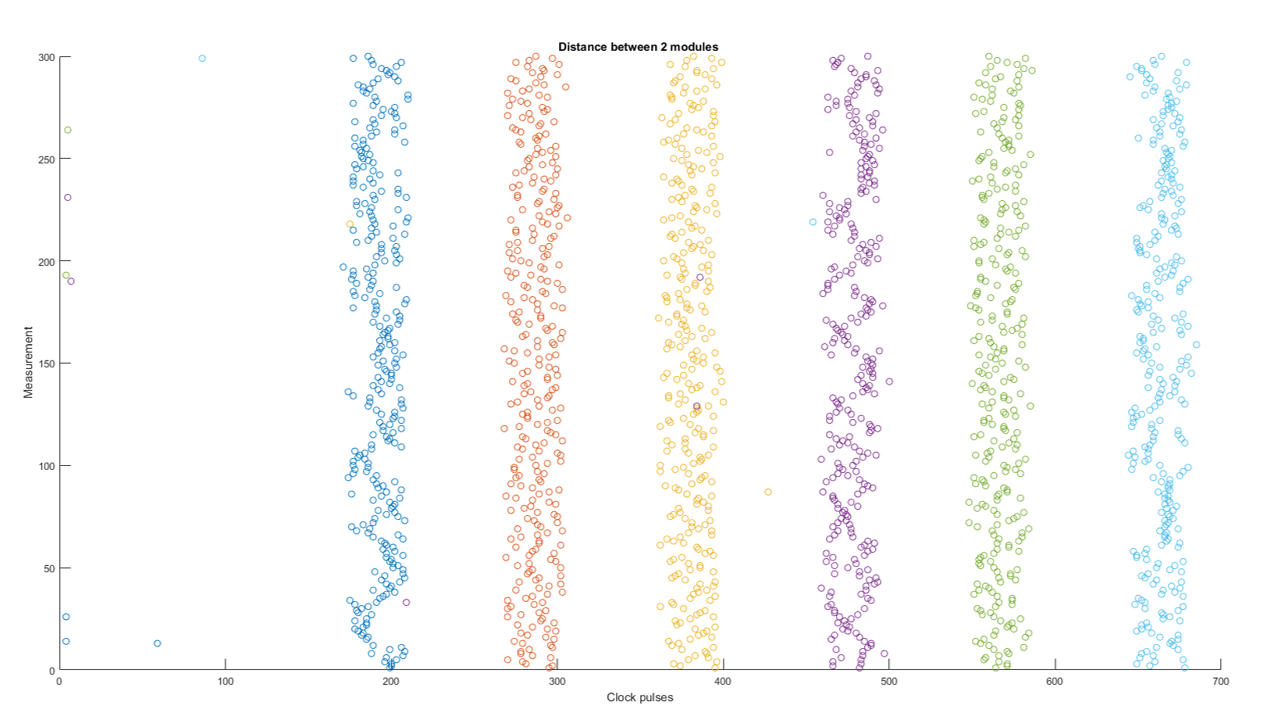
\includegraphics[width=0.9\textwidth]{Figures/Distance_6.png}
\caption{Measurement with static distances: \SI{1}{\meter},\SI{2}{\meter},\SI{3}{\meter},\SI{4}{\meter},\SI{5}{\meter} and \SI{6}{\meter}}
\label{fig:int_meas_1}
\end{figure}

There is a clear visible distinction between the measurements corresponding to the different distances in figure~\ref{fig:int_meas_1}.
Furthermore the spacing between the ``bands'' seems to be constant suggesting a linear relation between the measured number of clock cycles and the distances.
To further analyse the results the measurements of figure~\ref{fig:int_meas_1} are given as boxplots in figure~\ref{fig:int_meas_2}

\begin{figure}[H]
\centering
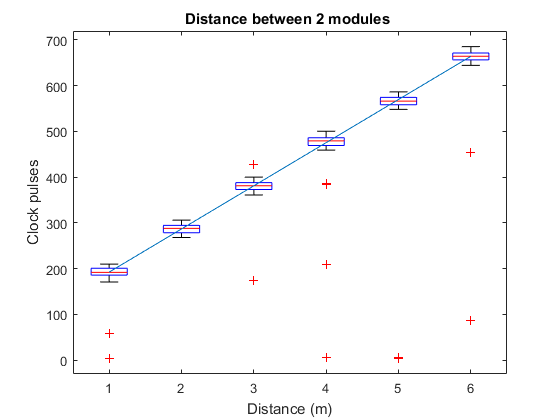
\includegraphics[width=0.8\textwidth]{Figures/Meas_1.png}
\caption{Boxplot representation of static measurements}
\label{fig:int_meas_2}
\end{figure}

From figure~\ref{fig:int_meas_2} the following conclusions are drawn:

\begin{itemize}
\item The relation between the measured number of clock cycles and the distances is linear as can be seen from the fitted line.
\item There are outliers but the differ a lot from mean of the measurements. We thus concludes that these can be easily rejected or filtered.
\item The error (deviation from mean) is constant for all distances. The error does not increase with a greater distance.
\item The error is roughly \SI{20}{\centi\meter} from the mean.
\end{itemize}

We thus draw the conclusion that the integrated system is capable of doing distance measurement between static modules.
With the next test the effect of multiple modules and moving modules is analysed.
Two modules are placed at static locations while the third is placed on a moving skateboard.
The resulting measurements are given in figure~\ref{fig:int_meas_3}.
Module 0 and Module 2 are the static modules, which is clearly visible in figure~\ref{fig:int_meas_3}.
Module 1 is the moving module as in figure~\ref{fig:int_meas_moving}.
In figure~\ref{fig:int_meas_3} this movement is clearly visible:

\begin{itemize}
\item First module 1 moves closer to module 0.
\item It then moves away farther from module 0.
\item Module 1 then moves closer to module 2.
\end{itemize}

This corresponds to the behaviour we expect with the set-up in figure~\ref{fig:int_meas_moving}.
We thus concludes that the systems works with multiple and moving modules.

\begin{figure}[H]
\centering
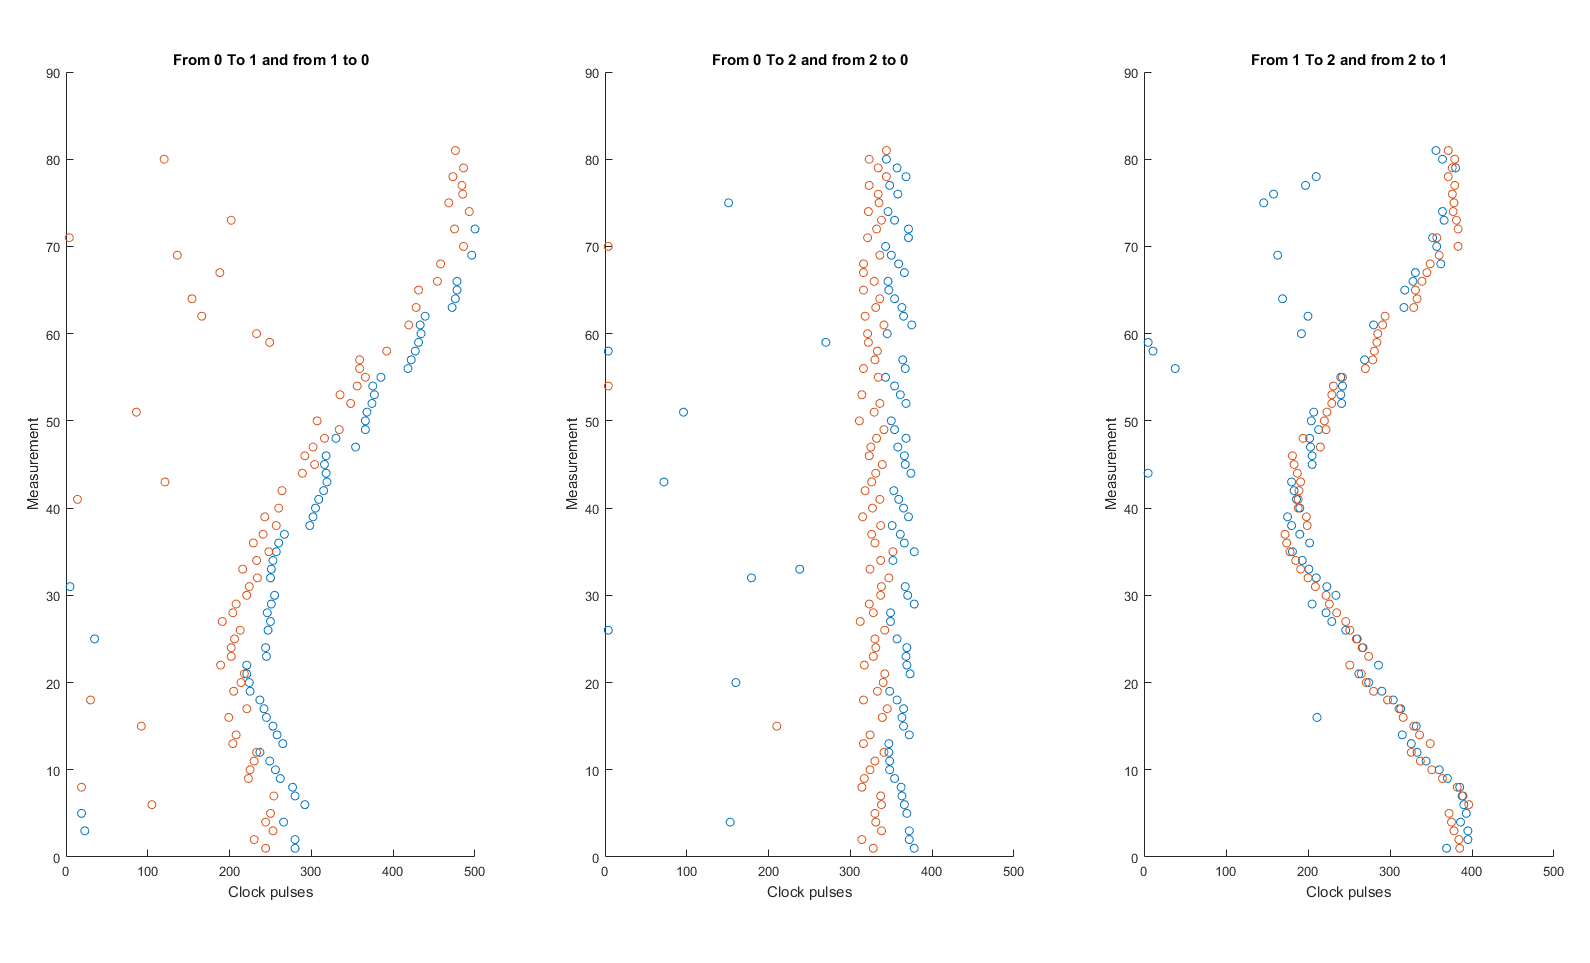
\includegraphics[width=0.9\textwidth]{Figures/meas_skate.png}
\caption{Measurements of moving modules}
\label{fig:int_meas_3}
\end{figure}

\begin{figure}[H]
\centering
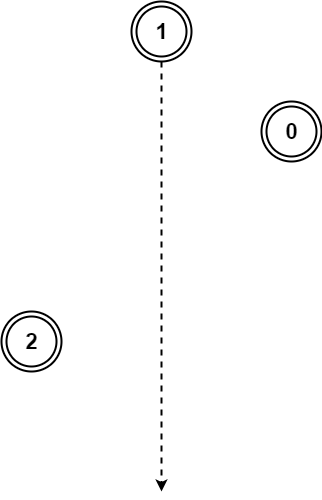
\includegraphics[width=0.4\textwidth]{Figures/moving_module.png}
\caption{Measurement set-up with moving module}
\label{fig:int_meas_moving}
\end{figure}

\chapter{Discussion}

As briefly discussed in chapter~\ref{chap:results} the accuracy of the results is low.
Since, at the time of writing, the prototype is not yet fully integrated measurements had to be done using an oscilloscope.
Using the oscilloscope in this set-up the resolution of the TDOA and delay measurements is \SI{0.1}{\milli\second}.
This corresponds to a distance resolution of \SI{3.4}{\centi\meter}.
In the final prototype these measurements will be done using a timer with a oscillator frequency of \SI{40}{\kilo\hertz} resulting in a resolution of \SI{25}{\micro\second}.
This resolution in time measurement gives a distance resolution of \SI{8}{\milli\meter}.
%By comparing these resolutions it's clear that, using the current results described in chapter~\ref{chap:results}, nothing can be said about the accuracy of the final fully integrated system.
%The results do show that even with the lower measurement resolution of the oscilloscope,
the required measurement resolution of \SI{10}{\centi\meter} from requirement~\ref{req:locres} is reached.

If we compare the resolution of \SI{8}{\milli\meter} to the error created by the uncertainty of the delay, \SI{17}{\centi\meter}, it's is clear that the final accuracy will be mainly determined by the uncertainty in the delay.
As discussed in chapter~\ref{chap:results} this error has a maximum of \SI{17}{\centi\meter} due to the Tx and Rx delay of the radio frequency pulse. Some imperfections of the antenna reflector result in an accuracy of \SI{20}{\centi\meter}.
This error is larger than the accuracy requirement \ref{req:locper} of \SI{10}{\centi\meter}.
This means that, without a filtering method the accuracy requirement is not met.

If we are able to characterise the distribution of the uncertainty in the delay the particle filter implemented on the MCU will be able to increase the accuracy.
How this particle filter works is discussed in~\cite{processing}.

In conclusion the results given in chapter~\ref{chap:results} do not give enough information to determine the final accuracy of the prototype system.
We can however make conclusions on which factors will have the largest influence on the accuracy.
The results do give enough data to conclude that the final system will be able to perform distance measurements with an accuracy close to the required performance.

The biggest limitation at this point in the project is the missing integration with the microcontroller.
If the microcontroller was integrated it would be possible to do a large set of measurement with a high resolution making it possible to draw conclusions on the accuracy of the system.
With the microcontroller integrated it is also possible to measure if the integration introduces an error.
As we've already seen the communication system had an unexpected large delay.
It could be possible that the integration with the microcontroller causes other delays.
At this point in time it is thus not possible to find all the delays in the complete system.

With the microcontroller present it is also possible to do better measurements on the communication channel delay.
It is important to characterize the distribution of the delay present in the communication channel to determine the average error introduced by the delay.
Currently only the max error is known (measured with a low resolution) but the average error can not yet be calculated.

If we want to fully test the prototype and draw meaningful conclusion about the accuracy of the prototype the full integration must be completed.
This full integration will be done in the final 2 weeks of the project which unfortunately means that they cannot be included in this thesis.
The steps required to complete this integration will be discussed in chapter~\ref{chap:recom}.

\chapter{Conclusion}
\label{chap:conc}
The first decision to be made was to, based on the state of the art research, decide on a concept.
The chosen concept is based on the Cricket project, a research project from MIT \cite{Priyantha2000,Priyantha2005,Balakrishnan2003,Smith2005}, and uses the following technique:
to measure the distance between Zebros a RF message and a ultrasonic pulse are transmitted concurrently, the distance between Zebros can than be calculated from the TDOA.
With this technique we reach the key performance indicators (KPI) as given in the programme of requirements:

\begin{itemize}
  \item
    \ref{req:neighbours} \textbf{The module should be able to locate multiple neighbouring Zebros (KPI).}
    As described in chapter~\ref{chap:concept} both the ultrasonic pulse and RF pulse reach all Zebros within the range of the ultrasonic pulse.
    The range of the ultrasonic pulse is larger than the required distance sensing range of \SI{5}{\meter} \ref{req:locrange}.
    This means that all Zebros within the required distance sensing range receive the necessary information to perform a distance measurement.
    As long as all Zebros get a turn to transmit their ultrasonic pulse and RF message all Zebros in the swarm can be located.
  \item
    \ref{req:allunits} \textbf{The module should be able to be used on and locate charging stations and similar units (KPI).}
    The chosen technique does not require modules to be moving in order to perform measurements.
    The module can thus be implemented on static objects such as a charging station.
  \item
    \ref{req:distinguish} \textbf{The module should be able to distinguish different users (Zebro, charging station, other member of Zebro familie) of the module (KPI)}
    The RF message, which is transmitted concurrently with the ultrasonic pulse, contains the Zebro serial number of the transmitting module.
    Using this serial number other Zebros know who is transmitting: it's tells them what the transmitter is (a Zebro, a charging station etc.) and who the transmitter is (Zebro 50 or Zebro 74).
    Thus the module can distinguish between different users.
\end{itemize}

After the conceptual design stage, we made some proof of concept circuits and 3D printed the antenna for the ultrasonic transceiver.
During tests we encountered some problems with the receiving circuit: the circuit had noise oscillations which were amplified and resulted in undesired outputs.
The problem was solved with the use of op-amp with a higher bandwidth.
Other problems occurred at the peak detection circuit, the capacitor discharged to fast resulting in undesired outputs of the comparator stages.
This problem was solved by changing the values of the components in the peak detection circuit.
With all circuit problems solved we were able to proof the correct working of the transmitter and receiver concepts.
The task after the proof of concept was to combine these transmitter and receiver circuit to a working prototype.

To make the working prototype, the module needed to switch between transmitting and receiving mode to protect the receiver part form the 30 $V_{p-p}$ of the transmitter.
Several options were available, but we decided to use an analogue switch, also called a bilateral switch, for this problem.
With all components known and proofed on, a naked prototype PCB was designed.
This prototype, made with a PCB milling machine, was used for integration and testing with the communication module.
A problem we encountered was that the module we used for sending and receiving the RF signal has a delay between transmission and receiving of a package.
We need to take this delay into account for determining the distance.

During the testing phase we found the results, with the delay taken into account, correspond to the actual distance between modules.
Since we use the average value of the delay we get an error corresponding to the deviation in the delay.
Using the delay gives a max. error of $\pm$ \SI{17}{\centi\meter}.
This means we do not comply to requirement \ref{req:locper} which states that the accuracy has to be at least \SI{10}{\centi\meter}

During these tests the processing method was not yet implemented.
Using the processing method, a particle filter, we might be able to increase the accuracy of the module.
As long as the distribution of the delay can be characterized, the particle filter will be able to improve the accuracy of the system.
Tests with the implemented particle filter will tell if the accuracy of the full system complies to requirement \ref{req:locper}.
These test will be performed after the deadline of the thesis.

The resolution of the measurements is \SI{8}{\milli\meter} since the TDOA is measured using a timer with a frequency of \SI{40}{\kilo\hertz}.
Requirement \ref{req:locres} states that the required resolution is \SI{10}{\centi\meter}.
This requirement is thus easily reached by the designed system.

We thus conclude that there is a high possibility that the fully integrated system will reach the requirements set by the Zebro team.
Before we can test the performance of the module work need to be done on the final integration of all systems.
We give a recommendation on the task required to finish the final integration in the next chapter.
These tasks will be undertaken by our project group in the last two weeks between the thesis deadline and the thesis defence.

\section{Conclusion after integration}

In chapter~\ref{chap:results} the results for the system after integration are given.
From these results we conclude that the integrated system (still without processing) is capable of performing distance measurements.
All the conclusions drawn above still hold for the integrated system, the accuracy is still the same.

\chapter{Recommendations}
\label{chap:recom}
Two types of recommendations are given:

The first type focusses on tasks necessary to integrate the full system and perform measurements.
These tasks are planned for the next two weeks and need to be completed before the module can be delivered to the Zebro team.
These recommendation are thus given as a list of tasks.

The second type of recommendations focusses on the future of the project.
How will the module fit into the Zebro project and how might the module change in the future of the Zebro project?
Possible improvements for the system will be discussed and topics which require more research are given.

\section{Tasks planned}

\begin{reqs}{R}
  \item
  Focus on integration of distance sensing systems with communication and processing system.
    \begin{subreqs}
      \item
      Connect distance sensing system to the microcontroller as described in section~\ref{sec:sys_int}.
      \item
      Implement counter measure for the delay in the communication channel as described in section~\ref{sec:delay}.
      \item
      Test if the microcontroller can calculate the TDOA of the ultrasonic pulse and the RF message.
    \end{subreqs}
  \item
  Focus on acquiring measurement results for full system.
    \begin{subreqs}
      \item
      Make testbench software which performs a large set of measurement for a single distance and stores the acquired results.
      \item
      Run tests for multiple distances.
      \item
      Analyse test results to determine accuracy and stability of fully integrated system.
    \end{subreqs}
  \item
  Focus on characterizing the distribution of the delay in the communication channel.
  \item
  Integrate module with Zebro power management system.
\end{reqs}

\section{Recommendations for the future of the module in the Zebro project}

With the tasks described above completed the module is ready to be implemented on the Zebro.
To check if the module works together small test have to be performed.
The most important of these test is to check if the module works on a waking Zebro.
It is possible that the movement of the leg influences the module performance.
If this is the case countermeasures can be taken.
The system can be calibrated or mechanically decoupled from the Zebro by using rubber dampeners in the mechanical connection.

It's possible that the reflector cone will become unstable when the Zebros moves at high speed or trough rough terrain.
If this happens it's possible to improve the stability by using 3 riser legs instead of 2.
During testing the effect of these risers on the transmitting and receiving behaviour was found to be negligible so using three risers will not affect the performance of the system.

More research could be done to improve the reflector antenna.
During the conceptual design the effect of material or the not completely smooth surface of the 3D print was not discussed.
It might be possible that a smooth metal reflector improves the transmitting and receiving behaviour antenna.

\subsection*{Zebro to the moon}

There are rumours of a Zebro going to the moon.
Our module does not work in the environment since we need the propagation of sound to do measurements.
If the Lunar Zebro requires a localization module we advise that research into an alternative to this module is performed as soon as possible.
During our state of the art research and conceptual design we found that most alternatives to the ultrasound system give poor performance.
RSSI for example has no direction relation to the distance between modules and is very dependent on device orientation.
Swarm networks further decrease the use of RSSI since the message are hopped in the network making it hard to find the RSSI value corresponding to a certain Zebro.
We believe that finding a working alternative to the system described in this paper requires time so we advice the Zebro team to look into alternative for the Lunar Zebro as soon as possible.
We estimate that the accuracy of these alternatives will be lower which has to be taken into account by the Zebro swarm behaviour group.


%----------------------------------------------------------------------------------------
%	APPENDICES
%----------------------------------------------------------------------------------------

\appendix % Cue to tell LaTeX that the following "chapters" are Appendices
%% Appendix A

\chapter{Frequently Asked Questions} % Main appendix title

\label{AppendixA} % For referencing this appendix elsewhere, use \ref{AppendixA}

\section{How do I change the colors of links?}

The color of links can be changed to your liking using:

{\small\verb!\hypersetup{urlcolor=red}!}, or

{\small\verb!\hypersetup{citecolor=green}!}, or

{\small\verb!\hypersetup{allcolor=blue}!}.

\noindent If you want to completely hide the links, you can use:

{\small\verb!\hypersetup{allcolors=.}!}, or even better: 

{\small\verb!\hypersetup{hidelinks}!}.

\noindent If you want to have obvious links in the PDF but not the printed text, use:

{\small\verb!\hypersetup{colorlinks=false}!}.

% Appendix A
 % For referencing this appendix elsewhere, use \ref{AppendixA}
\chapter{KiCad Circuits}
\label{Appendixcircuits}
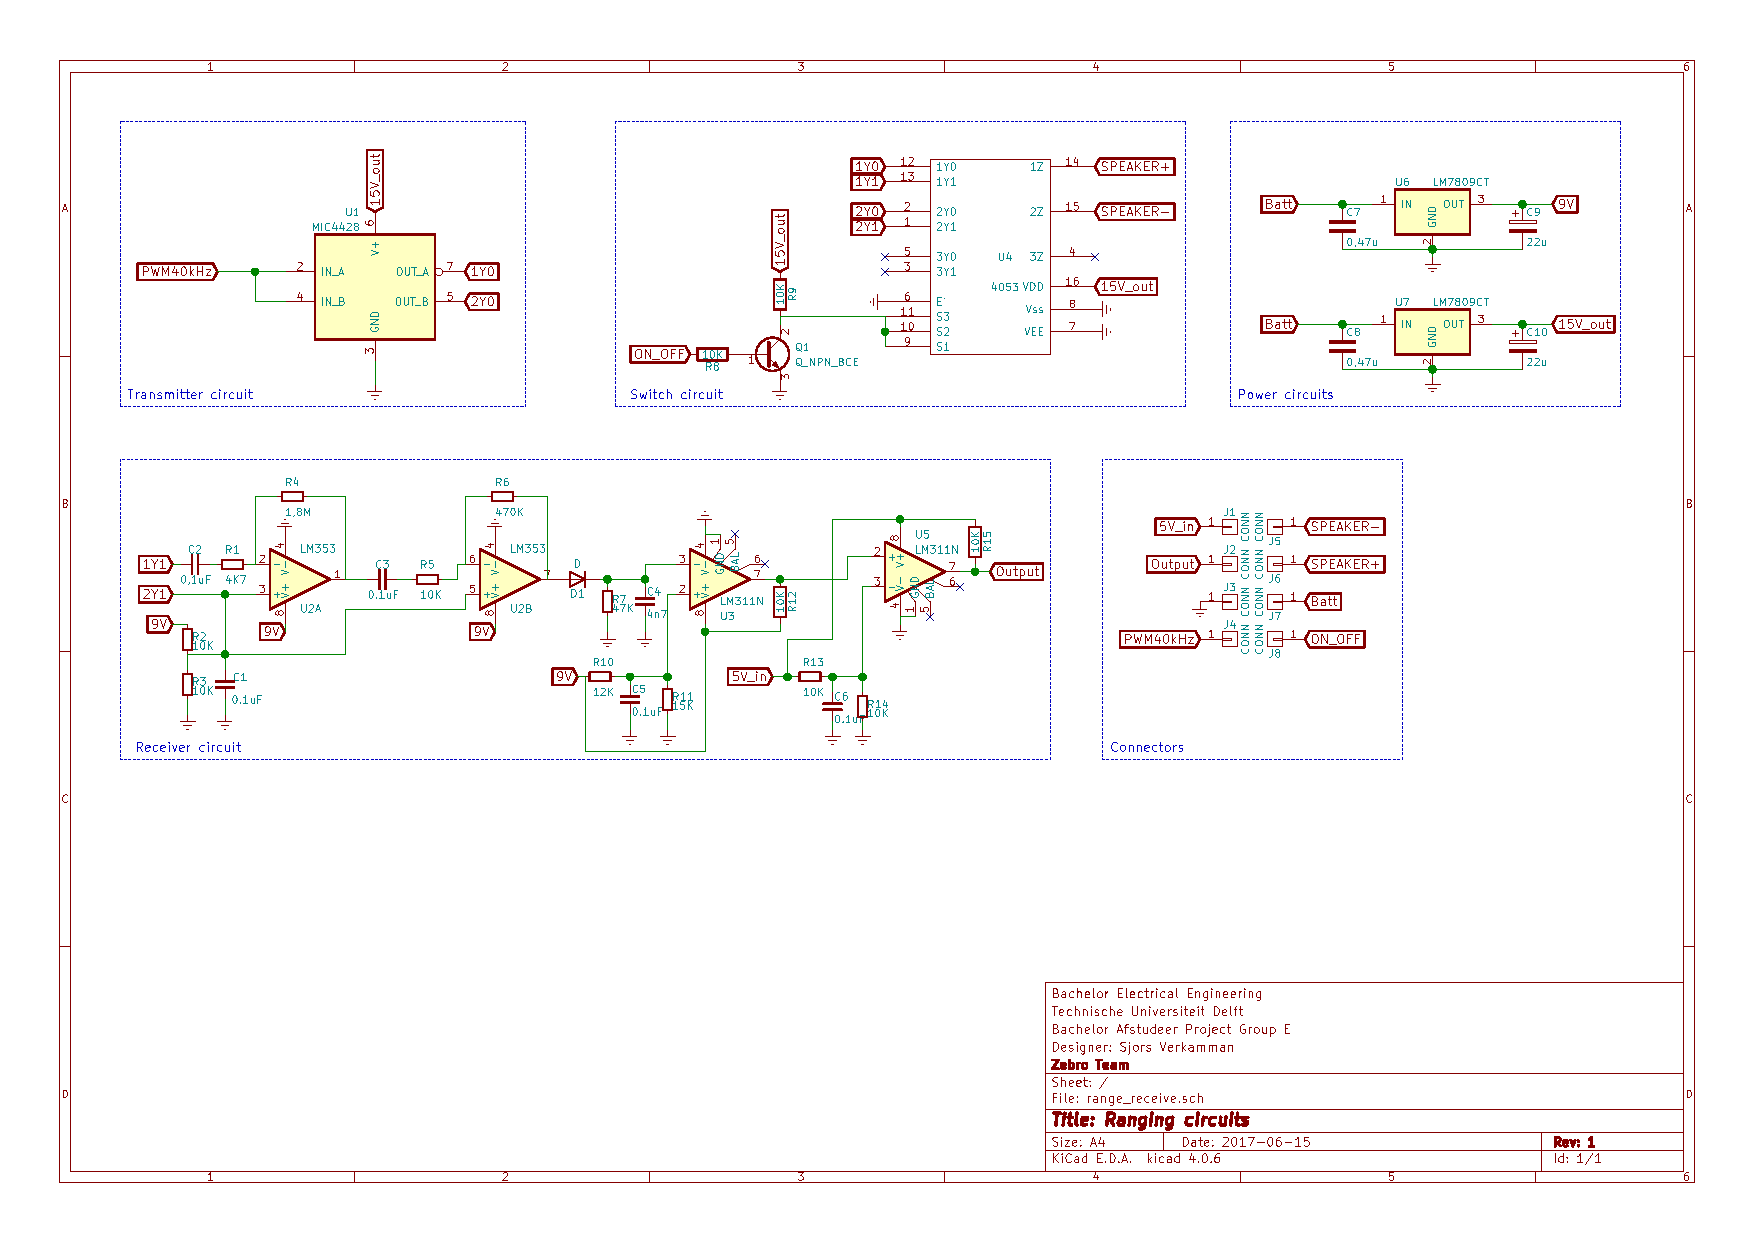
\includepdf[landscape=true]{PDFfiles/range_receive.pdf}

% Appendix A


%\label{AppendixBOM} % For referencing this appendix elsewhere, use \ref{AppendixA}

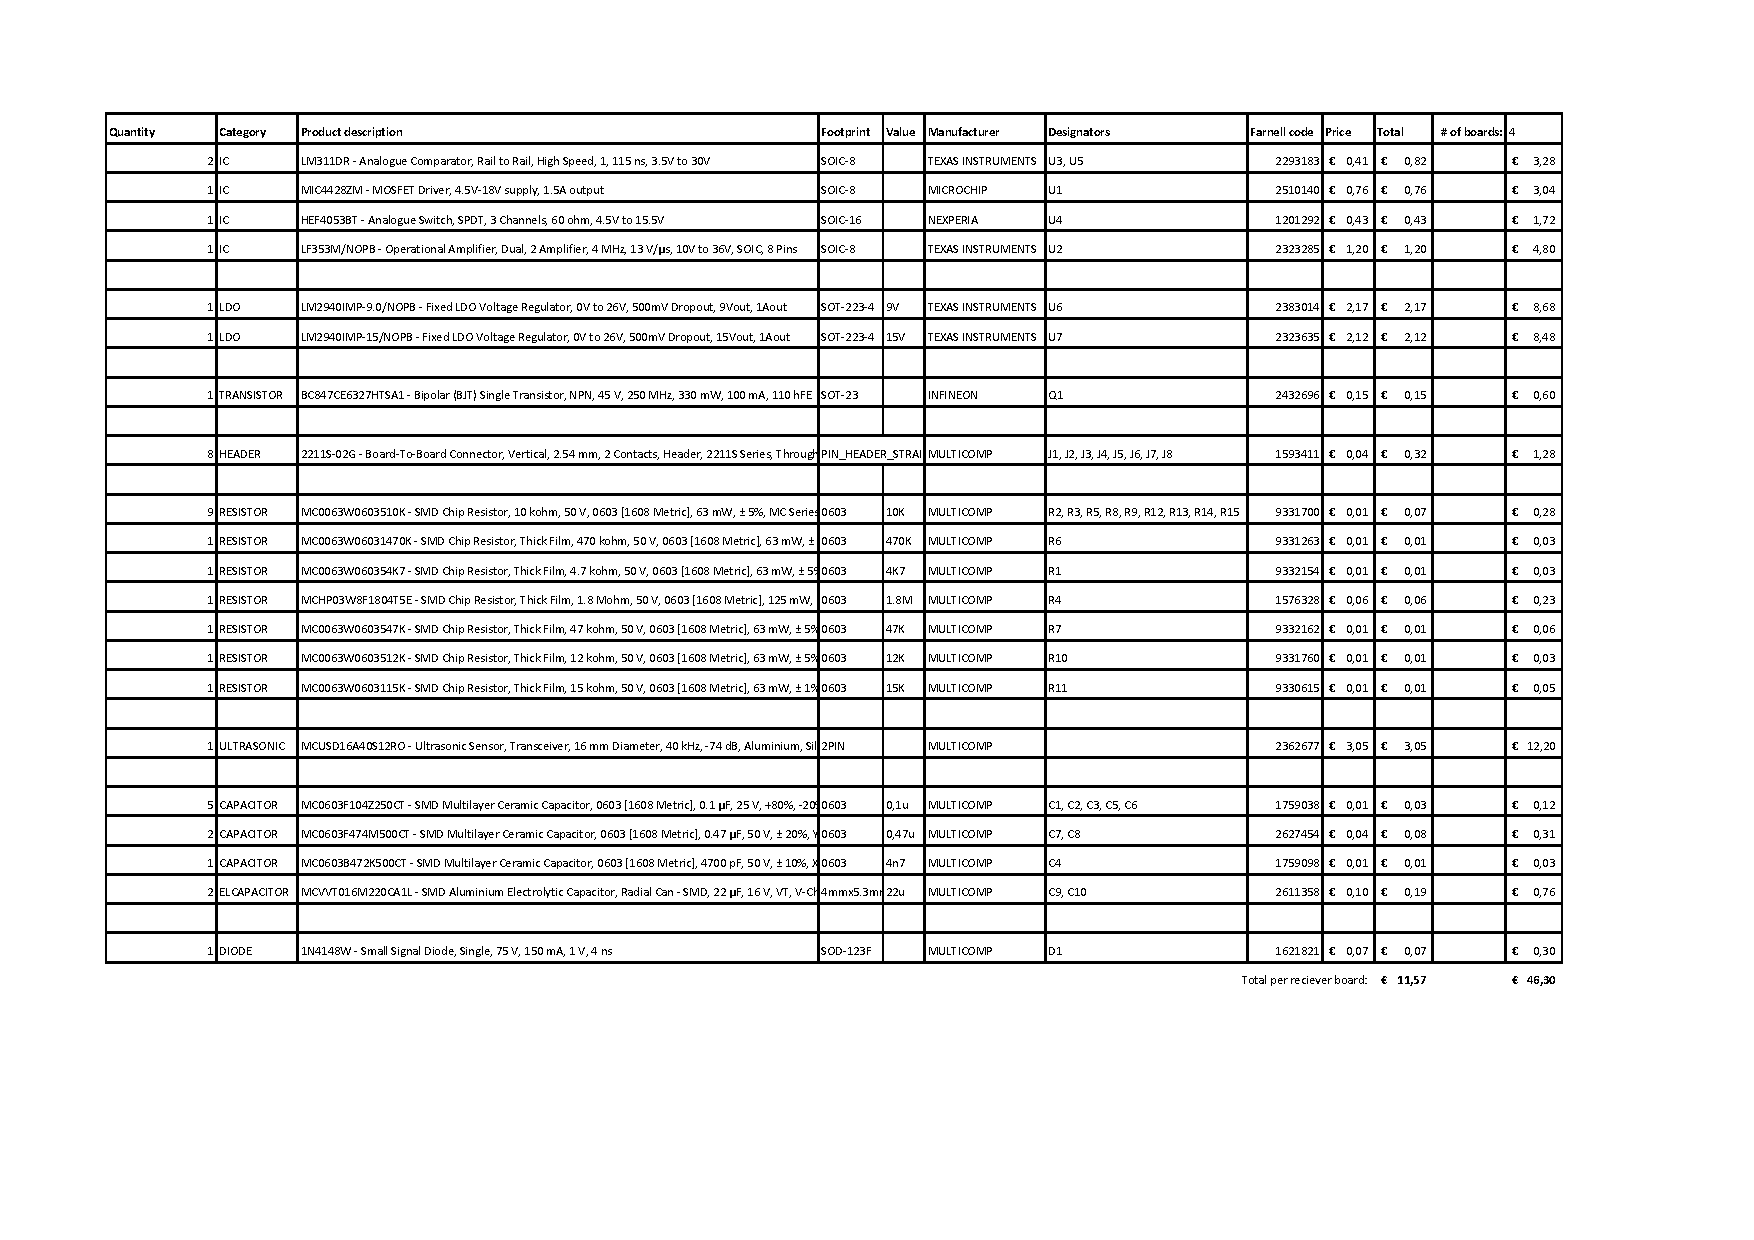
\includepdf[pages=1,pagecommand=\chapter{Bill of Materials}\label{AppendixBOM}]{PDFfiles/BOM_ranging.pdf}


%----------------------------------------------------------------------------------------
%	BIBLIOGRAPHY
%----------------------------------------------------------------------------------------
\printbibliography[heading=bibintoc,title={Bibliography}]{}
%----------------------------------------------------------------------------------------

\end{document}
